\chapter{The High-Luminosity LHC}
\label{chap:hllhc}

\section{Introduction}
The obvious means for improving precision measurements is to take more data. Run 2 of the LHC finished in 2018, delivering p-p collisions at $\sqrt{s}=13$~TeV and reaching a maximum instantaneous luminosity of around $2\times10^{34}$~\lumi. After a shutdown period for upgrades and maintenance, Run 3 is expected to commence in 2022 and finish in 2024. Here, the LHC machine will operate with an instantaneous luminosity of $2\times10^{34}$~\lumi over the full data-taking period, at $\sqrt{s}=13$ or $14$~TeV. By the end of Run 3, over $\mathcal{L}=300$~\fbinv of p-p collision data will have been collected by the CMS experiment.

Since the statistical uncertainty in a measurement scales according to $1/\sqrt{\mathcal{L}}$, simply operating with the same beam conditions beyond Run 3 is not particularly interesting; the machine would have to run for many years to see a worthwhile improvement in the precision. A future operation of the LHC machine, referred to as the High-Luminosity LHC (HL-LHC)~\cite{ApollinariG.:2017ojx}, will upgrade the LHC beam and therefore maximise the physics potential. During this phase, proton bunches will be collided at $\sqrt{s}=14$~TeV, with a nominal instantaneous luminosity of $5\times10^{34}$~\lumi, rising to as high as $7.5\times10^{34}$~\lumi towards the end of operation. Scheduled to begin in 2027, this means by the mid-2030s an integrated luminosity of around 3000~\fbinv (3~\abinv) will be available for physics analysis. Not only will this dramatically reduce the statistical uncertainty in existing measurements, but it will also open the door for new measurements and analyses that are not possible with a limited dataset. One such example is provided in section \ref{sec:trilinear}, looking at the potential of constraining the Higgs boson self coupling using ttH~+~tH differential measurements.

Unfortunately, the increase in the instantaneous luminosity comes at a price. At the HL-LHC, the mean pileup per bunch crossing is expected to be as high as 200. This poses a major challenge both in terms of the higher radiation levels delivered to the LHC experiments, and the ability to trigger on and reconstruct physics objects of interest in a high pileup environment. As a result, all LHC experiments will undergo major upgrade programmes to accommodate the HL-LHC conditions. The operation of the CMS detector during the HL-LHC is referred to as CMS Phase-2. For this operation, the CMS experiment will not only replace the existing parts of the detector with high levels of radiation damage, but will improve the functionality of these parts in terms of the radiation hardness and the granularity~\cite{Contardo:2020886}. Amongst the numerous upgrades, two of the most substantial developments are with respect to the L1T and the endcap calorimeters~\cite{CERN-LHCC-2017-023,CERN-LHCC-2020-004}.

The design latency of the CMS Phase-2 L1T will be extended to 12.5~$\mu$s. This enables the use of more granular information from the various subdectors in the trigger decision including, for the first time, hits in the inner tracker. Advances in Field Programmable Gate Array (FPGA) technology~\cite{Duarte_2018}  will also facilitate more complex algorithms at the L1T stage, including the application of a Particle-Flow-like algorithm to link the various subdetectors, as well as machine learning (ML) algorithms such as Boosted Decision Trees (BDTs). Furthermore, the combined improvements in the front-end electronics and the data acquisition (DAQ) system~\cite{CERN-LHCC-2017-014} allow the maximum output event rate of the L1T to be increased to 500~kHz. All in all, these upgrades are crucial for maintaining an excellent trigger efficiency in a high pilueup environment.

By the end of Run 3, the CMS endcap calorimeters will be significantly radiation damaged, such that their performance will be substantially reduced. For Phase-2, the ECAL and HCAL endcaps will be completely replaced by a single subdetector, known as the High Granularity Calorimeter (HGCAL), which will have both electromagnetic and hadronic components. The HGCAL will exhibit a fine segmentation in both the transverse and longitudinal directions, as well as timing capabilities, to enable the precise reconstruction of both electromagnetic and hadronic showers in four dimensions. This is an extremely exciting prospect for studying physics processes in the forward region, such as reactions initiated by vector boson fusion (VBF) and those with highly boosted objects.

\section{The High Granularity Calorimeter}\label{sec:hgcal}
The design of the HGCAL~\cite{CERN-LHCC-2017-023} is driven mainly by the need to be radiation tolerant and maintain a good energy resolution over the full lifetime of the HL-LHC project, as well as exhibiting sufficient granularity to perform calorimetry in the forward region; a schematic of this design is provided in Figure~\ref{fig:cms_hgcal}. It will cover the pseudorapidity region: $1.5<\eta<3$, and  consist of an electromagnetic compartment (CE-E), followed by a hadronic compartment (CE-H). The design is comprised mainly of silicon detector technology, which has been shown to withstand and perform well in the high particle-flux environment. This is supplemented with plastic scintillator tiles towards the rear of the detector, where the scintillation light is read out by silicon photo-multiplier tubes. The active material of the detector is interleaved with layers of lead and stainless steel absorber, which increases the effective depth of the calorimeter and thus provides good containment of the particle showers.

\begin{figure}[htb!]
  \centering
  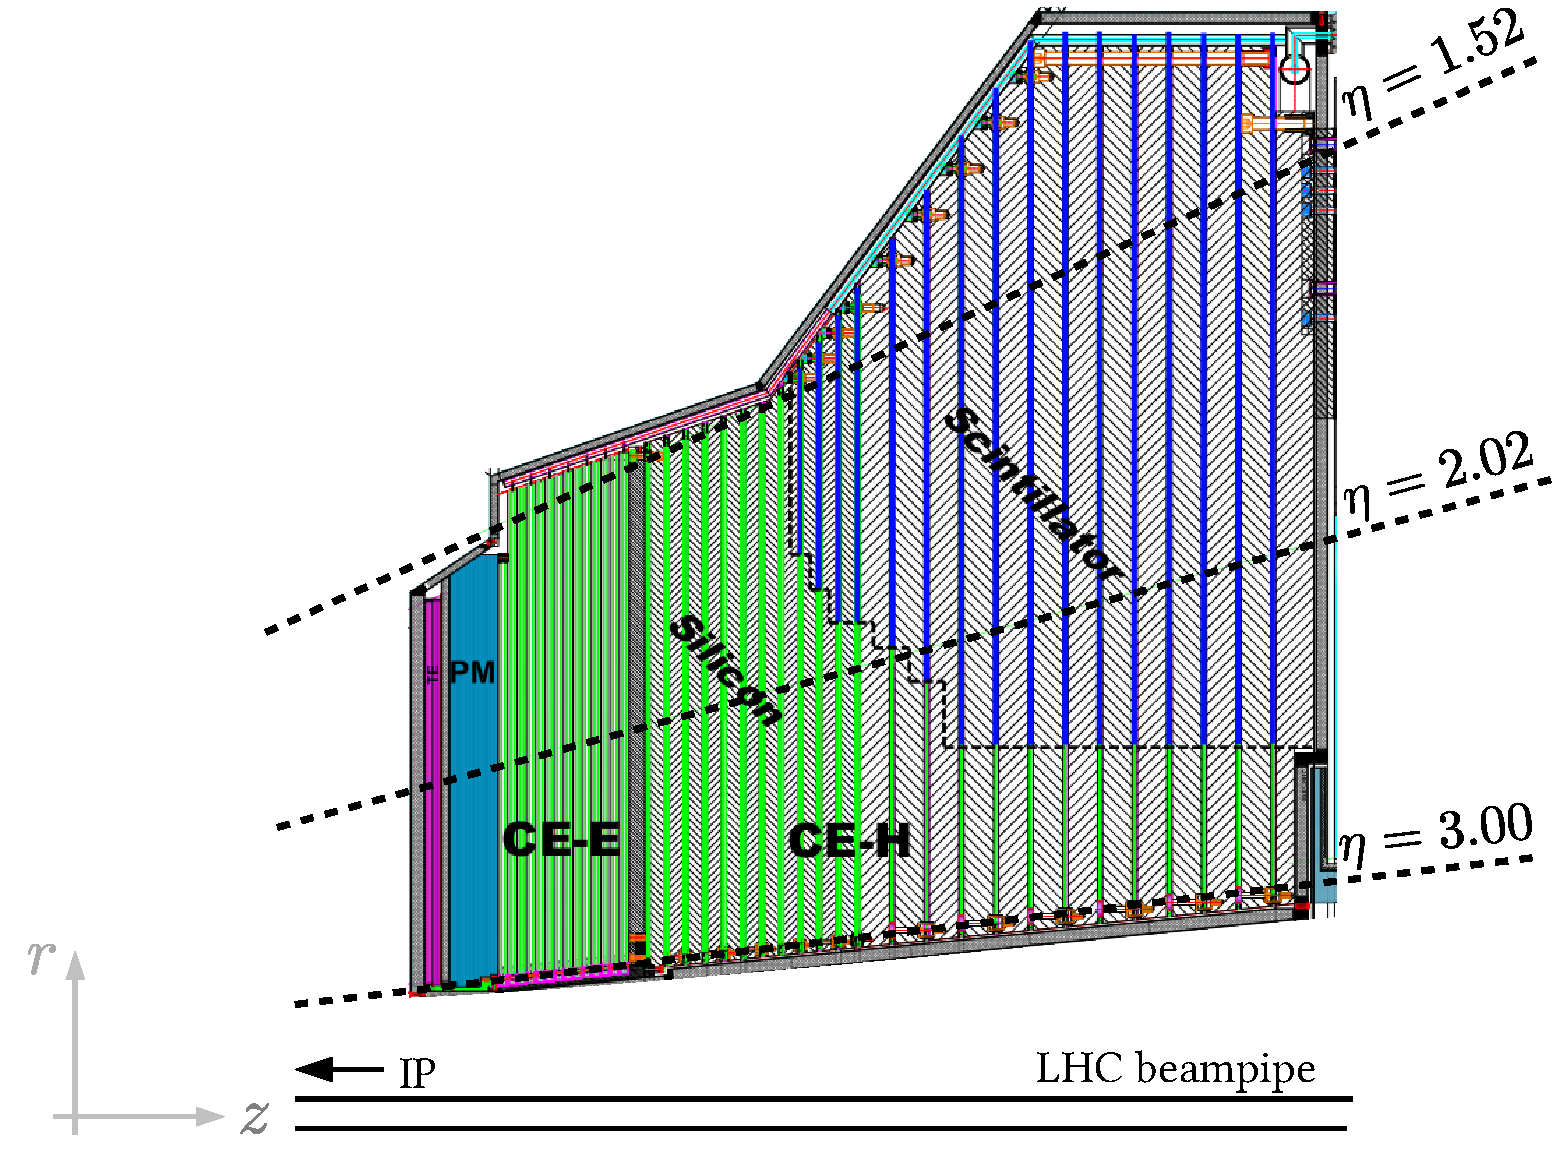
\includegraphics[width=1\textwidth]{Figures/cms/hgcal.pdf}
  \caption[Longitudinal structure of the High-Granularity Calorimeter]
  {
    Longitudinal structure of the HGCAL. The electromagnetic compartment (CE-E) consists of 28 sampling layers, interleaved with hexagonal silicon sensors (green). The total depth of the CE-E is 26 radiation lengths ($X_0$) and 1.7 nuclear interaction lengths ($\lambda_I$). The hadronic compartment (CE-H) is formed of 24 sampling layers, with an increased thickness for the rear 12 layers. The active material in this region is composed of silicon sensors (green) and plastic scintillator (blue), for the region of the detector with lower levels of radiation. The CE-H extends the total depth of the HGCAL to 10.7~$\lambda_I$. In front of the CE-E lies the endcap timing layer (TE, purple) which aids in the mitigation of pileup, and a polythene neutron moderator (PM) layer to reduce the neutron flux in the CE-E. Figure has been adapted from that shown in Ref.~\cite{CERN-LHCC-2017-023}.
  }
  \label{fig:cms_hgcal}
\end{figure}

The HGCAL will feature unprecedented transverse and longitudinal segmentation. Both the silicon sensors and the plastic scintillator tiles will be highly segmented, with a size of $\approx0.5-1$~cm$^{\rm{2}}$ and $\approx4-30$~cm$^{\rm{2}}$, respectively. Coupling this property, with the fact that the highly dense material in the HGCAL leads to laterally compact showers, enables excellent shower separation. Moreover, fine lateral granularity limits the region used for the shower energy measurement and thus minimises the energy enhancement from particles originating in pileup interactions. The longitudinal segmentation of 28 layers in the CE-E and 24 layers in the CE-H provides a handle on the longitudinal development of a particle  shower. This capability, which is not possible in the current CMS calorimeters, improves the electromagnetic energy resolution, enables pattern recognition, and helps to mitigate showers originating from pileup. Finally, the intrinsic timing capabilities of the silicon sensors means that each energy deposit can be given a precise time stamp. This timing information is especially useful for pileup rejection, identification of the interaction vertex, and for the PF reconstruction.

% All of these attributes make the HGCAL an extremely powerful component for the CMS Phase-2 physics programme. Being in the forward region, the HGCAL will be key for triggering and reconstructing processes initiated by Vector Boson Fusion (VBF) and those including highly-boosted objects. The superb shower separation and pattern recognition capabilities will help identify narrow jets (e.g. from $\tau$'s) or merged jets (e.g. from the hadronic decays of boosted W and Z bosons). Finish physics goals!

An extra design requirement of the HGCAL is the ability to contribute to the L1T decision.
%, particularly for the signatures of the aforementioned processes of interest. 
As introduced in the previous section, advances in FPGA technology enables the application of more complex and powerful algorithms at the L1T stage. The remainder of this section is dedicated to a machine learning (ML) algorithm designed to differentiate electrons and photons from jets in the HGCAL L1T. Before going into the specific details, it may benefit the reader to refresh themselves with the introduction to ML algorithms is section~\ref{sec:ml_algo}.

\section{Electron and photon identification in the HGCAL L1T}\label{sec:egid}
The high granularity of the HGCAL enables electromagnetic showers originating from single electrons or photons ($e/\gamma$) to be resolved, even in the very high occupancy environment of the HL-LHC. To successfully reconstruct events containing such objects, it is necessary to correctly identify $e/\gamma$ showers at the L1T decision stage. This section investigates the application of a BDT to distinguish $e/\gamma$ candidates (signal) from pileup-induced clusters (background) in the HGCAL L1T. For the studies, dedicated MC simulation samples are used which correspond to collisions in the CMS Phase-2 detector with a centre-of-mass energy of $\sqrt{s}=14$~TeV and an average of 200 pileup interactions per event.

Despite the increased total latency of the CMS Phase-2 L1T allowing HGCAL information to be used, it is not possible to read out the data with full granularity. To reduce the data, only alternate layers in the CE-E are used, and neighbouring silicon sensors (scintillator tiles) are summed into so-called \textit{trigger cells} with a granularity of approximately 4~cm$^{\rm{2}}$ (16-100~cm$^{\rm{2}}$). Additionally, a reasonably tight energy threshold is placed on the trigger cells and no timing information is stored. A clustering algorithm~\cite{CERN-LHCC-2020-004} is applied to the selected trigger cells, which (in a similar fashion to the algorithm described in section \ref{sec:particle_flow}) first seeds the clusters and then builds topological clusters around these identified seeds. The resulting 3D clusters form the collection of HGCAL \textit{trigger primitives}, on which the L1T decision is based. Even with the data reduction techniques, the trigger primitives contain sufficient information regarding the 3D development of the particle shower to efficiently identify $e/\gamma$ candidates and reject clusters originating from pileup.

The \textsc{XGBoost} software package~\cite{10.1145/2939672.2939785} is used for BDT training, where the input data are simulated HGCAL trigger primitives (3D clusters). Input features ($\vec{x}$) are the five longitudinal and four lateral shower shape variables listed in table~\ref{tab:egid_features}. The energy weighted RMS features are defined for generic trigger cell co-ordinate, $p$, as,
\begin{equation}
    {\rm{Weighted}\,\,\rm{RMS}}(p) = \sqrt{\frac{1}{E_{\rm{tot}}}\sum^{N_{\rm{tc}}}_{i} E_i (p_i-\langle p \rangle)^2}\,
\end{equation}
\noindent
where the sum is over a collection of trigger cells, each with energy, $E_i$, and co-ordinate, $p_i$. The quantity $\langle p \rangle$ is the energy weighted mean of $p$ over the whole collection, whilst $E_{tot}=\sum^{N_{\rm{tc}}}_iE_i$. Features of this type give an indication of the shower spread in the $p$ co-ordinate direction.

In the training, signal clusters are identified as those consistent with originating from a generator-level electron of $p_T > 20$~GeV\footnote{This is done by requiring the reconstructed cluster to be within an angular separation of $\Delta R<0.2$ with a generator-level electron.}, where the cluster is required to pass a minimum $p_T$ threshold of 10~GeV. Note, only electron clusters are required for training the $e/\gamma$ identifier since both photon and electron showers have almost identical features in the HGCAL. Background clusters (pileup) are all clusters with $p_T>20$~GeV that are not matched to a generator level electron. 

\begin{table}[htb!]
    \caption[HGCAL L1T $e/\gamma$ identification BDT input features]{Input features to the HGCAL L1T $e/\gamma$ identification BDT.}
    \label{tab:egid_features}
    % \vspace{.5cm}
    \centering
    \scriptsize
    \renewcommand{\arraystretch}{2}
    \hspace*{-1.5cm}
    \begin{tabular}{r|p{0.65\textwidth}}
    \hline
    \multicolumn{2}{c}{\textbf{Longitudinal shower shape variables}} \\ \hline
    Weighted RMS($z$) & Energy weighted RMS of trigger cell $z$ co-ordinate, evaluated over the whole cluster. Measure of the longitudinal spread of the shower. \\
    First layer & First layer of the HGCAL with an energy deposit (above the trigger cell threshold). \\
    Max layer &  Layer of the HGCAL with maximum cluster energy deposit. \\
    Shower length & Total length of the cluster calculated as the difference between the first layer and the last layer with an energy deposit. \\
    Core shower length & Maximum number of consecutive layers with energy deposits in the cluster. \\
    \hline
    \multicolumn{2}{c}{\textbf{Lateral shower shape variables}} \\ \hline
    Weighted RMS($r$) & Energy weighted RMS of trigger cell $r$ co-ordinate, evaluated over the whole cluster. The $r$ co-ordinate is divided by the $z$ co-ordinate in the calculation to account for the spreading out of the shower as it propagates through the HGCAL. Measure of the radial spread of the shower. \\
    Mean layer weighted RMS($r$) & Energy weighted RMS of trigger cell $r$ co-ordinate, evaluated for each layer separately, and averaged over the whole cluster. Again, the $r$ co-ordinate is divided by the $z$ co-ordinate to account for the spreading out of the shower. Measure of the radial spread of the shower. \\
    Weighted RMS($\eta$) & Energy weighted RMS of trigger cell $\eta$ co-ordinate, evaluated over the whole cluster. Measure of the polar angle spread of the shower. \\
    Weighted RMS($\phi$) & Energy weighted RMS of trigger cell $\phi$ co-ordinate, evaluated over the whole cluster. Measure of the azimuthal spread of the shower.\\
    \hline
\end{tabular}
    \hspace*{-1.5cm}
\end{table}

Two separate BDTs are trained in the pseudorapidity regions, $1.5<|\eta|<2.7$ and $2.7<|\eta|<3.0$, to account for the fact that the $e/\gamma$ shower shape features evolve rapidly as a function of $\eta$. This improves the overall background rejection with respect to training a single BDT inclusive in $\eta$, particularly in the high $|\eta|$ region. Figure~\ref{fig:egid_features} shows the Max layer (longitudinal) and Weighted RMS($\eta$) (lateral) distributions for signal and background clusters in each $\eta$ region. Both features show good discriminating power. The Max layer distribution demonstrates that most $e/\gamma$ showers deposit their maximum energy in the CE-E compartment (first 28 layers, where only alternate layers contribute to the trigger primitive), whilst clusters originating from pileup are more likely to deposit their maximum energy in the CE-H compartment (back 24 layers). The distributions of all input features are shown in Appendix~\ref{app:egid_features}.

\begin{figure}[htb!]
  \centering
  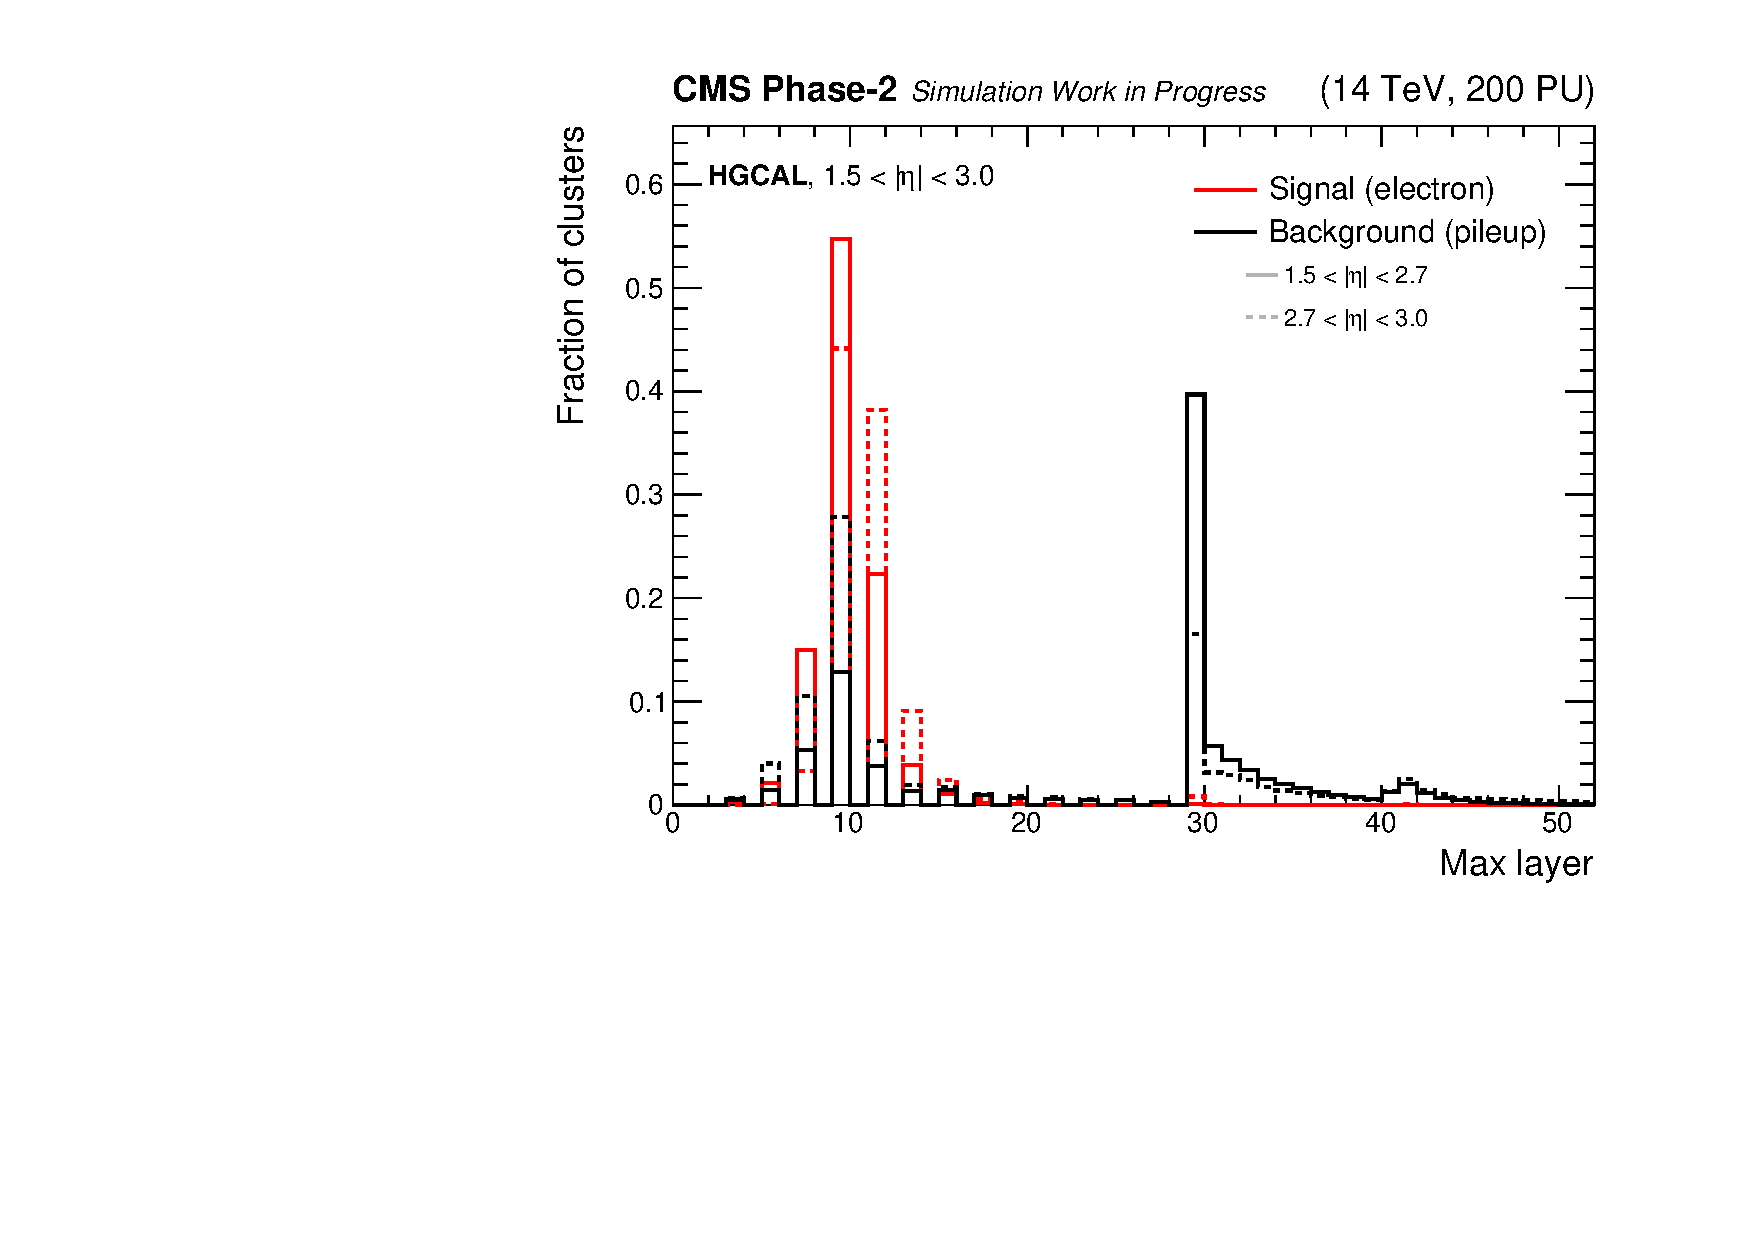
\includegraphics[width=.49\textwidth]{Figures/cms/egid/cl3d_maxlayer.pdf}
  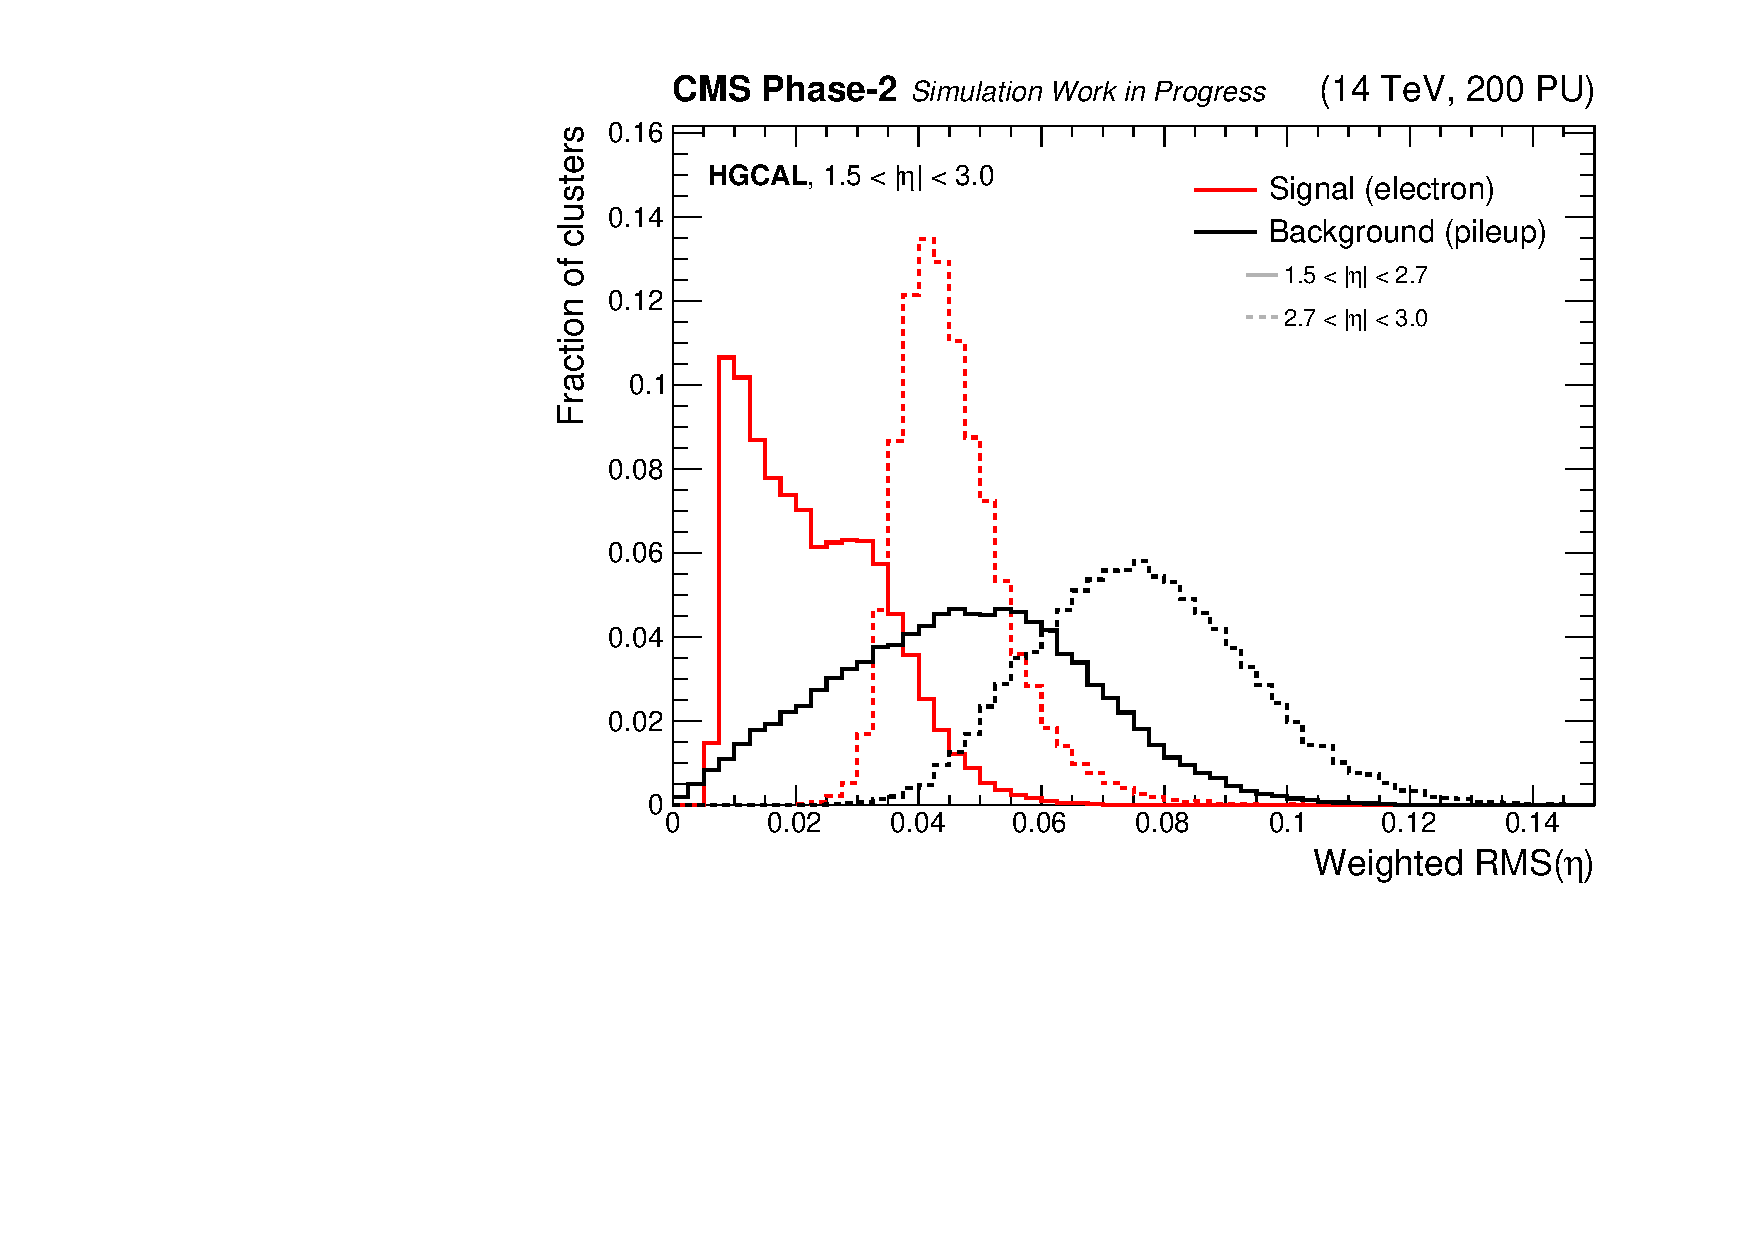
\includegraphics[width=.49\textwidth]{Figures/cms/egid/cl3d_seetot.pdf}
  \caption[$e/\gamma$ identification input feature distributions]
  {
    The Max layer (left) and Weighted RMS($\eta$) (right) distributions for signal and background clusters, separated into the two pseudorapidity regions.
  }
  \label{fig:egid_features}
\end{figure}

\subsection{Performance}
The \textit{output score} distributions of the two BDTs are shown for signal and background clusters in Figure~\ref{fig:egid_output}; the scores are effectively a measure of how signal-like (1) or background-like (-1) the clusters are based on the input shower shape features, $\vec{x}$. 

\begin{figure}[htb!]
  \centering
  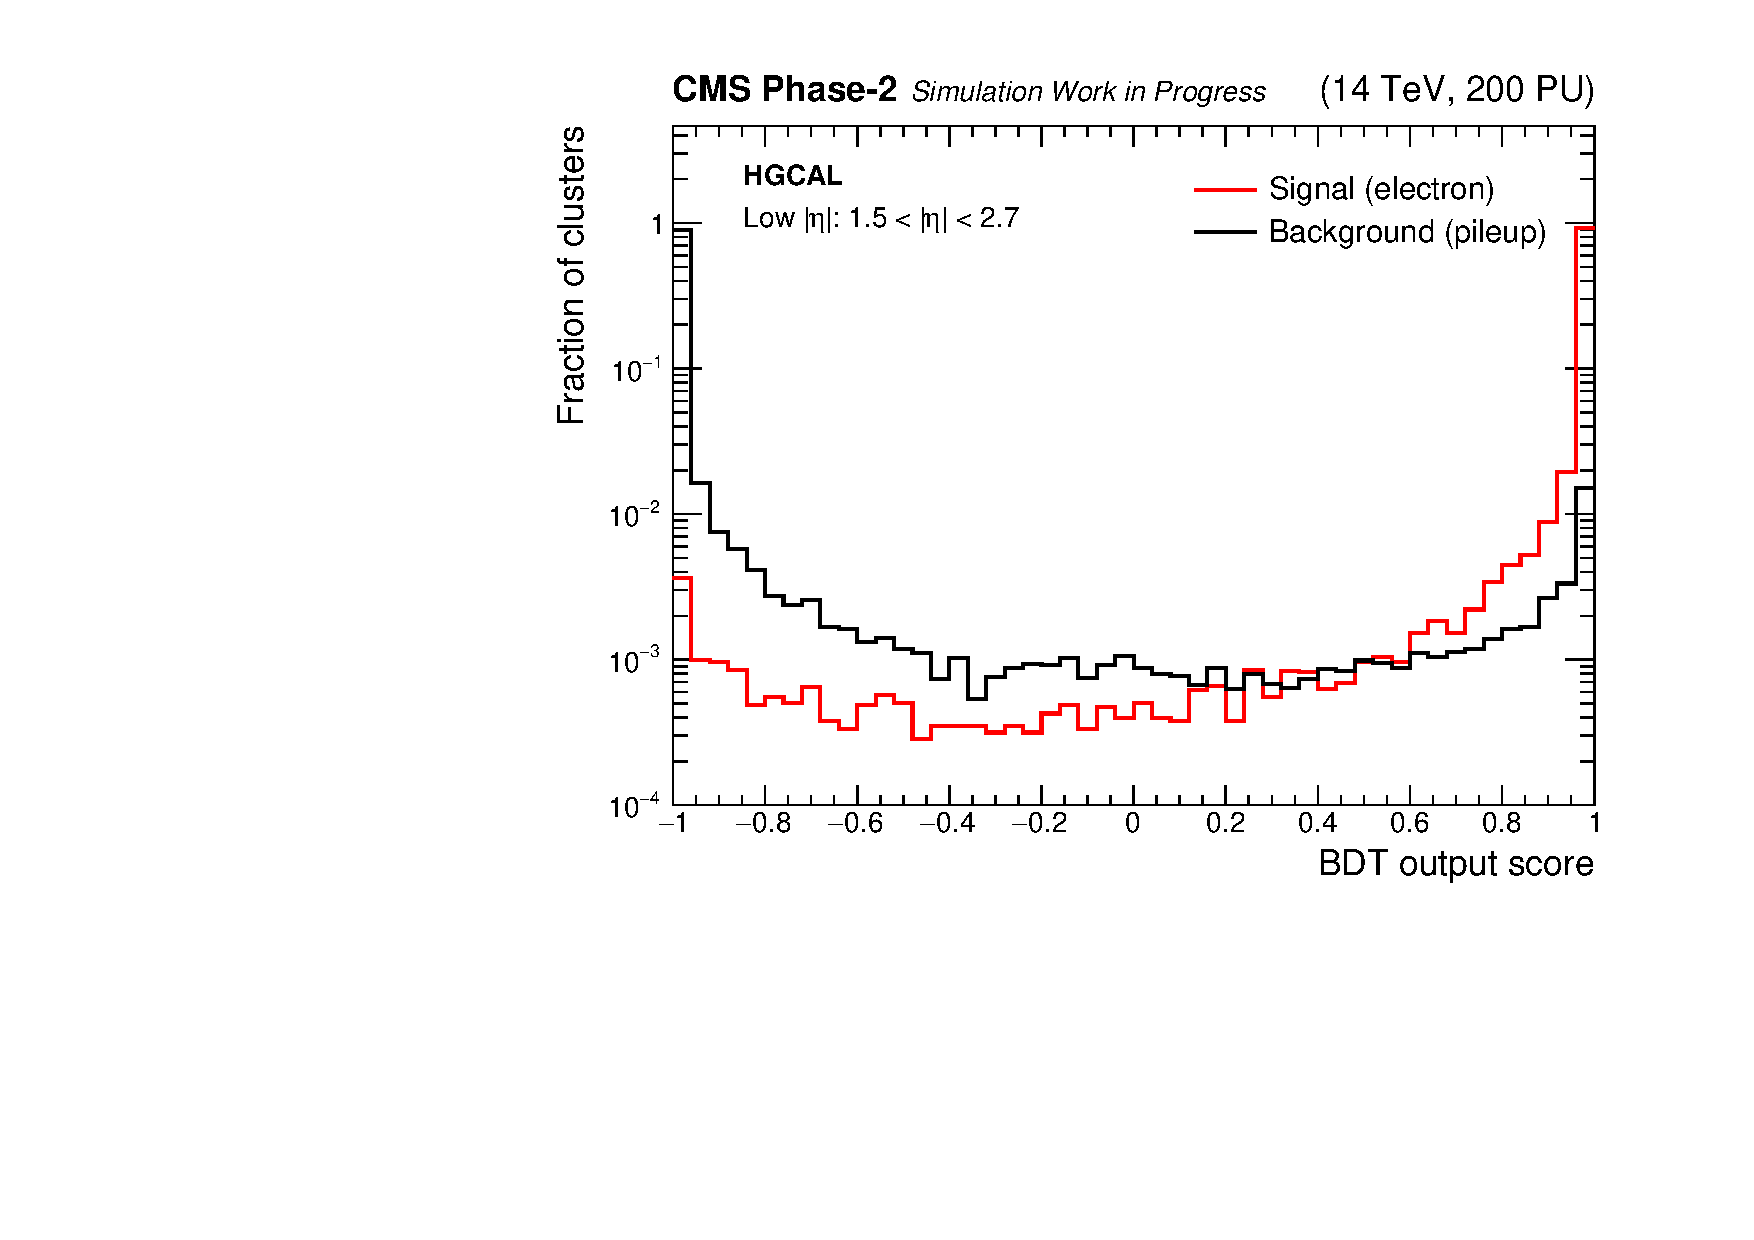
\includegraphics[width=.49\textwidth]{Figures/cms/egid/cl3d_bdt_electron_200PU_vs_neutrino_200PU_full_lo.pdf}
  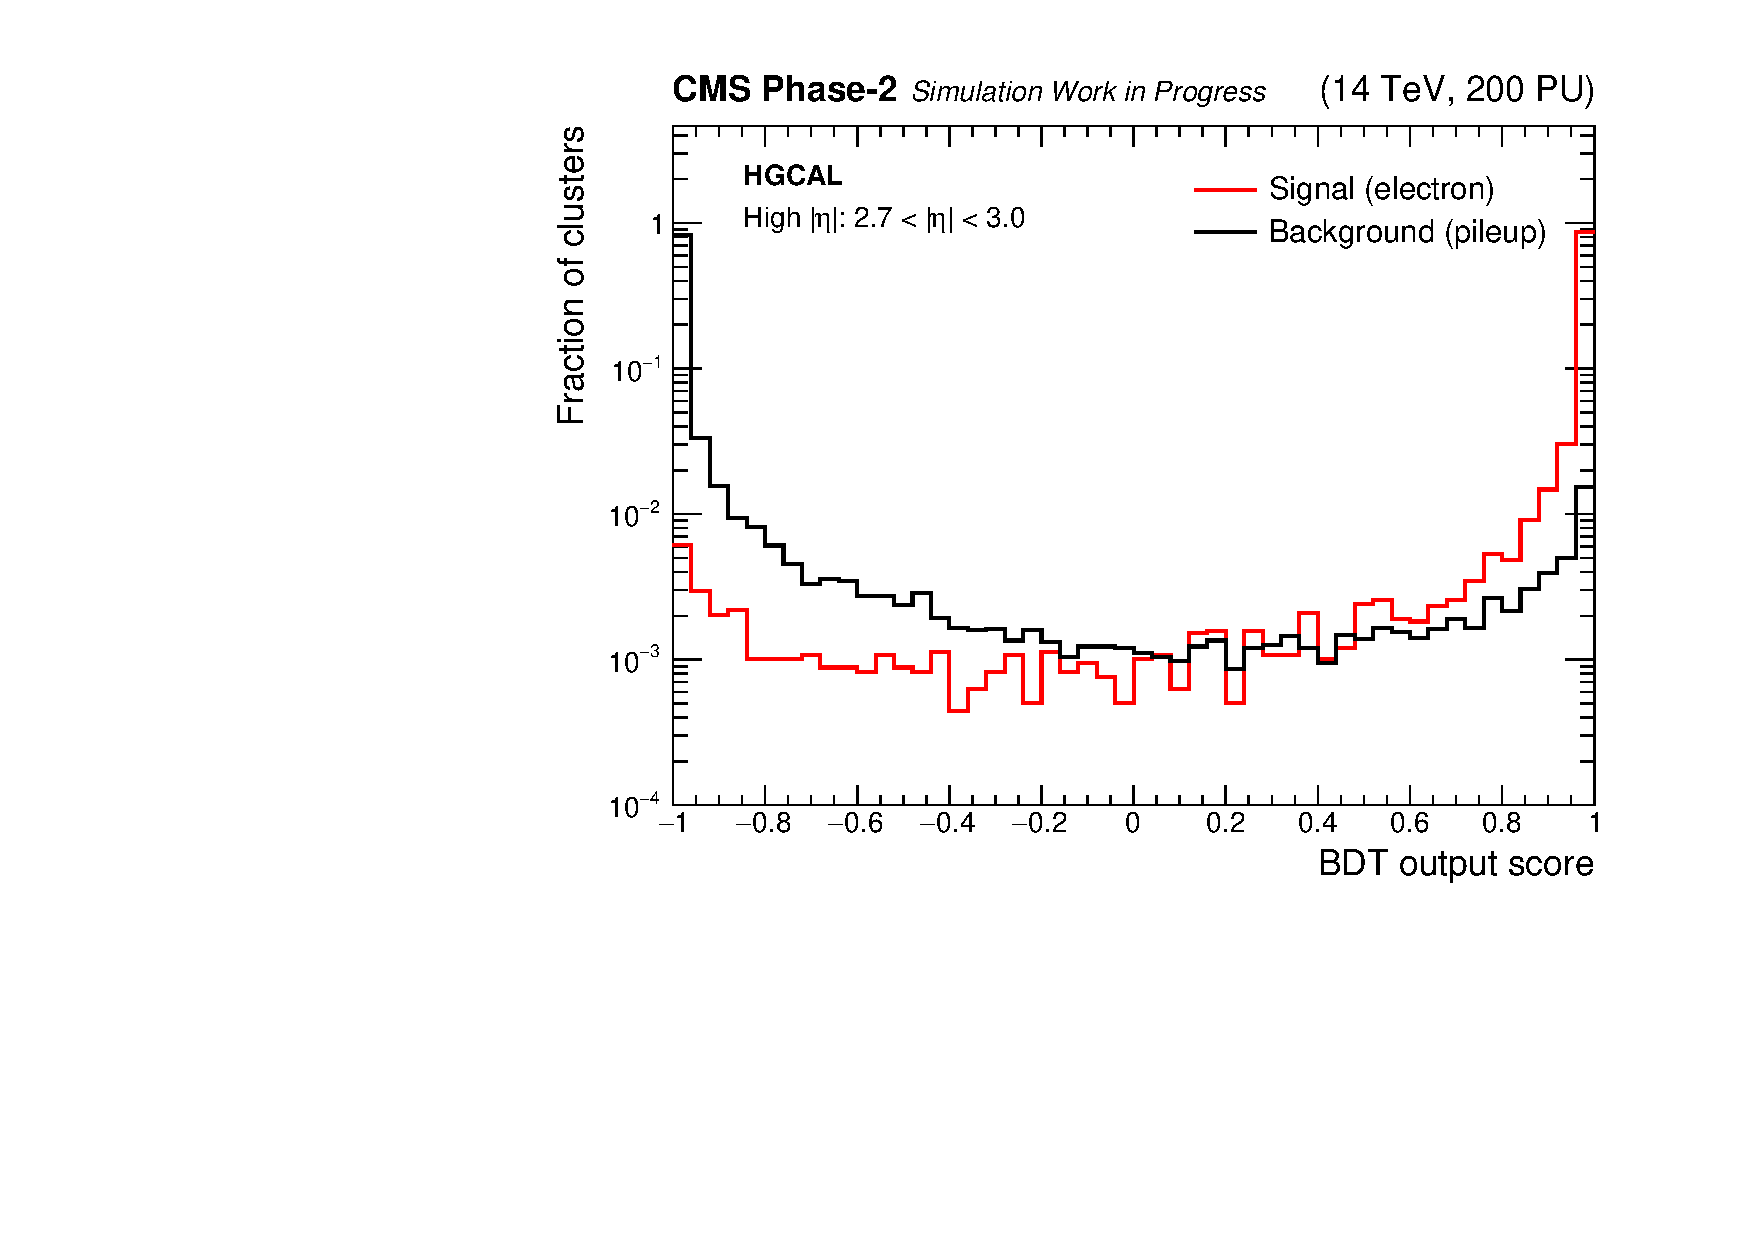
\includegraphics[width=.49\textwidth]{Figures/cms/egid/cl3d_bdt_electron_200PU_vs_neutrino_200PU_full_hi.pdf}
  \caption[$e/\gamma$ identification output score distributions]
  {
    BDT output score distributions for signal and background clusters. The BDT trained in the low $|\eta|$ region ($1.5<|\eta|<2.7$) and the BDT trained in the high $|\eta|$ region ($2.7<|\eta|<3.0$) are shown in the left and right plots, respectively. The outputs show excellent discrimination between signal and background clusters.
  }
  \label{fig:egid_output}
\end{figure}

The performance of the classifier is evaluated using the area under the receiver operating characteristic (ROC) curve~\cite{roc}. Each point in the ROC curve corresponds to the signal efficiency and background rejection evaluated at a given threshold on the BDT output score. Here, the signal efficiency is defined as the fraction of generator-matched electron clusters above the BDT output score threshold, whilst the background rejection is defined as the fraction of pileup clusters rejected at the same threshold. The ROC curves, evaluated using an independent test sample, are shown for both BDTs in Figure~\ref{fig:egid_roc}. The performance is shown to be slightly better for the low $\eta$ region. 

\begin{figure}[htb!]
  \centering
%   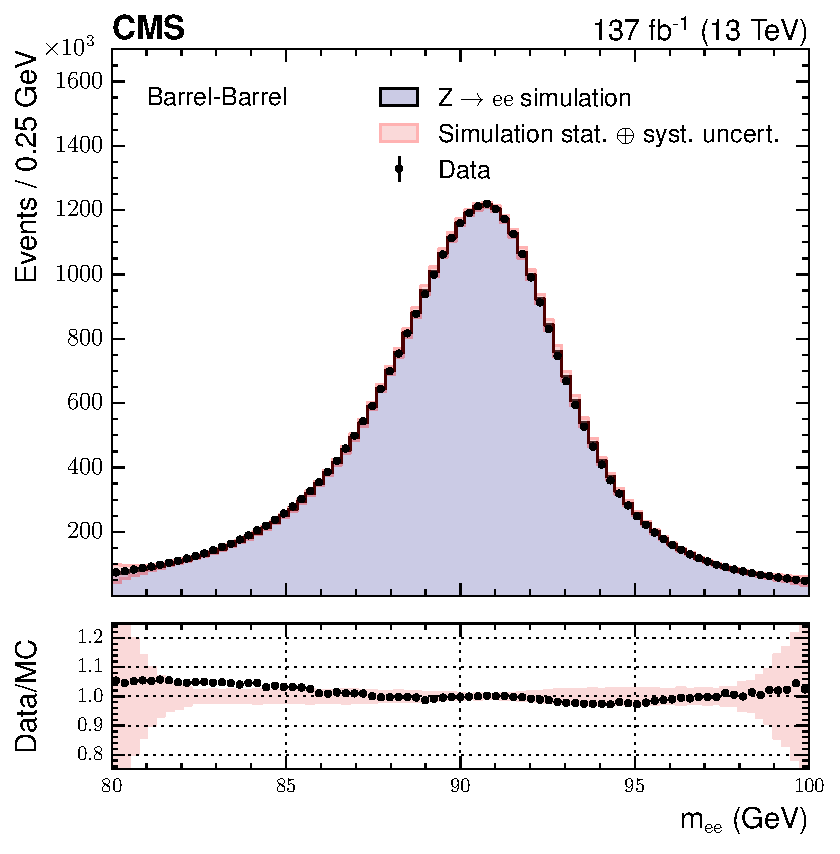
\includegraphics[width=.45\textwidth]{Figures/hgg_overview/money_run2_EbEb_inclusive.pdf}
  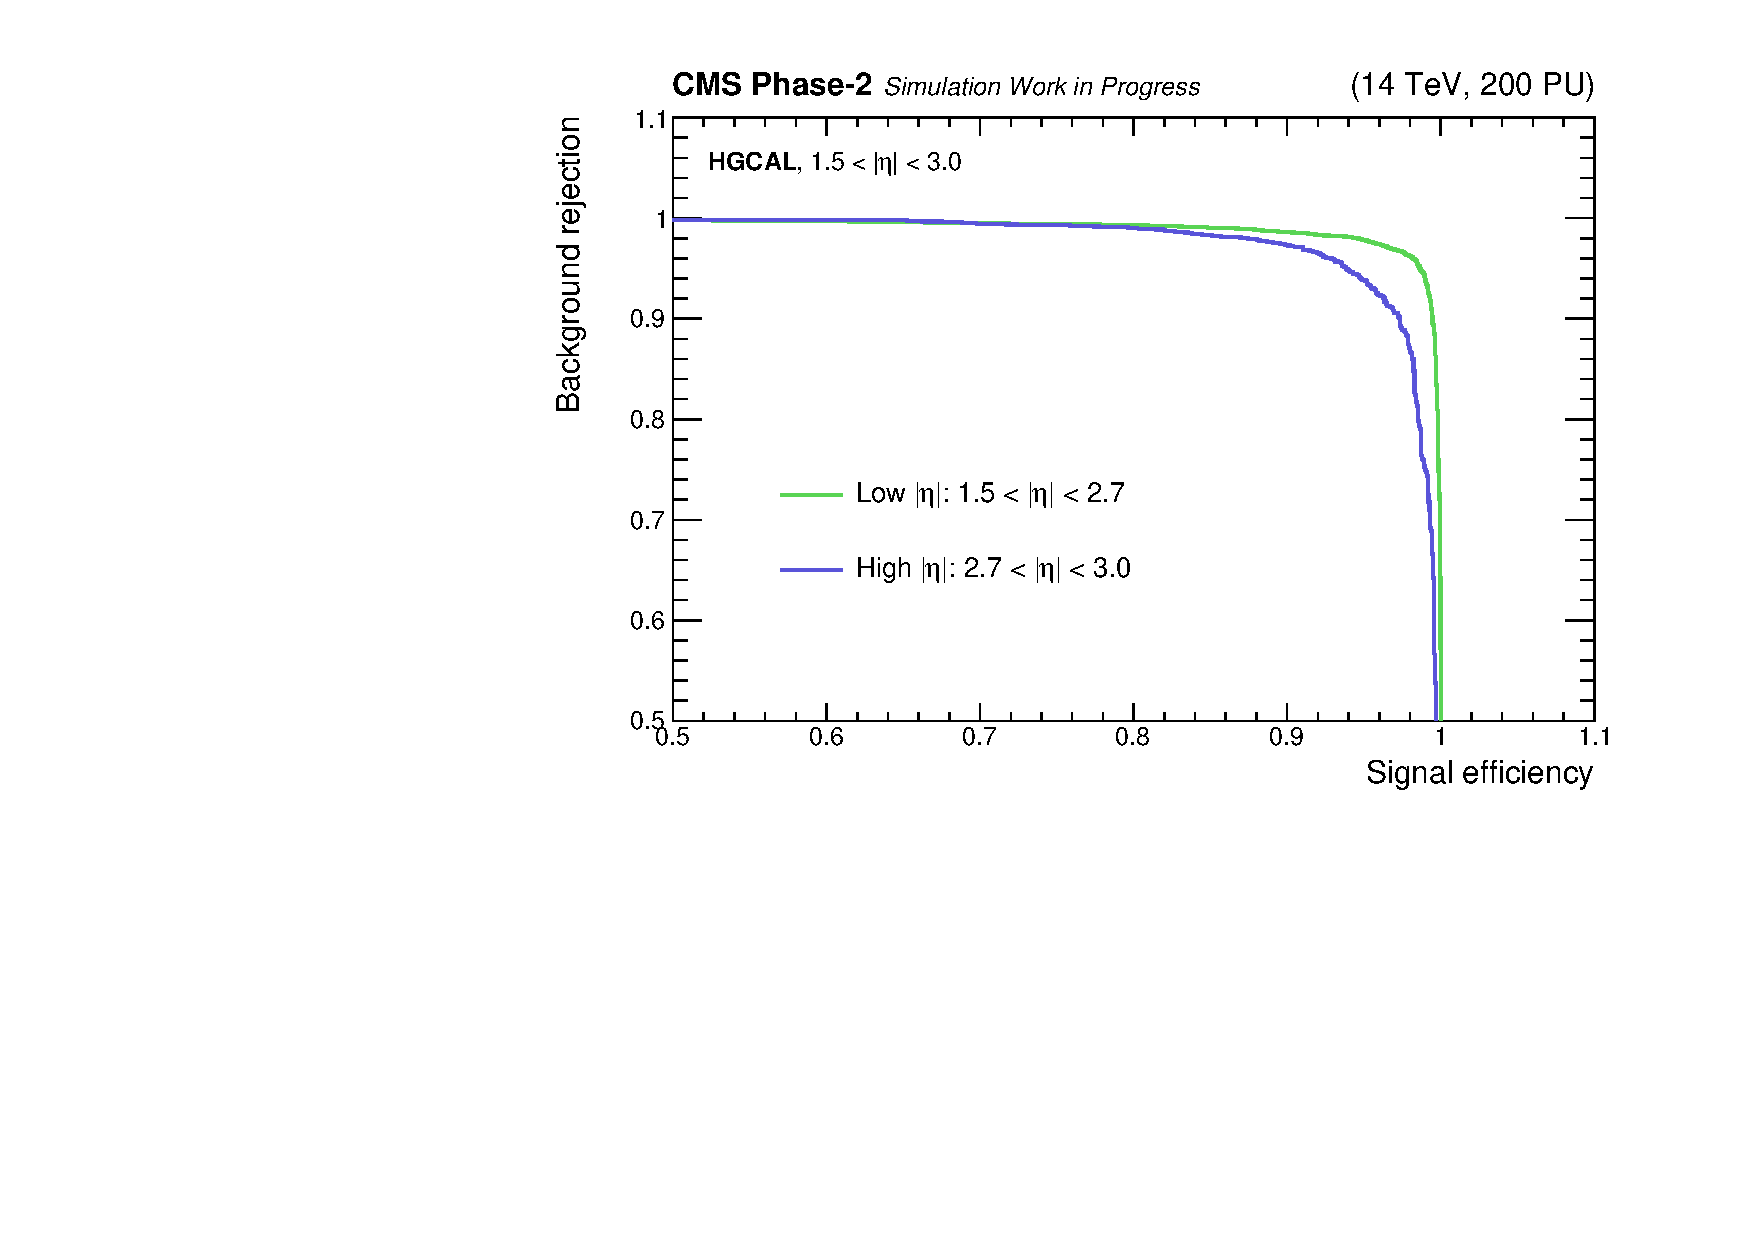
\includegraphics[width=.7\textwidth]{Figures/cms/egid/ROC.pdf}
  \caption[$e/\gamma$ identification ROC curve]
  {
    ROC curves for the $e/\gamma$ identification BDTs, trained in the low $|\eta|$ region ($1.5<|\eta|<2.7$, green) and the high $|\eta|$ region ($2.7<|\eta|<3.0$, blue).
  }
  \label{fig:egid_roc}
\end{figure}

Baseline thresholds on the output scores (working points) are chosen for an inclusive signal efficiency of 97.5\% in the $1.5<|\eta|<2.7$ region and 90.0\% in the $2.7<|\eta|<3.0$ region. These correspond to background rejections of 96.7\% and 97.3\%, respectively. The tighter working point for high $|\eta|$ is chosen to combat the increased levels of pileup in this region. Ultimately, the excellent discriminating power is a result of the highly segmented design of the HGCAL, which provides a powerful handle on the lateral and longitudinal development of particle showers.

The trigger efficiency of the algorithm is shown as a function of the generator level electron $p_T$ and $|\eta|$ in Figure~\ref{fig:egid_efficiency}. This efficiency is defined as the fraction of generator level electrons with $p_T>30$~GeV that:
\begin{itemize}
    \item have a matching trigger primitive cluster separated by an angle $\Delta R<0.2$ with respect to the generator level electron, where the cluster is required to have a reconstructed $p_T>20$~GeV \textit{and} pass the aforementioned working points on the $e/\gamma$ identification BDT.
\end{itemize}
\noindent
In the plots, the grey lines indicate the fraction of electrons with a matching cluster; this is practically 100\% for all pseudorapidity bins, except the two at the HGCAL edges where the electron can fall outside of acceptance. The blue lines then indicate the efficiency after applying the $e/\gamma$ identification working points. It is shown to increase as a function of electron $p_T$, rising from 94\% at $p_T=30$~GeV to around 99\% for $p_T=100$~GeV. Also, the efficiency is shown to decrease with increasing electron $|\eta|$, barring the first pseudorapidity bin. This is especially noticeable in the high $|\eta|$ region ($2.7<|\eta|<3.0$) where a tighter working point is applied on the BDT output score.

\begin{figure}[htb!]
  \centering
  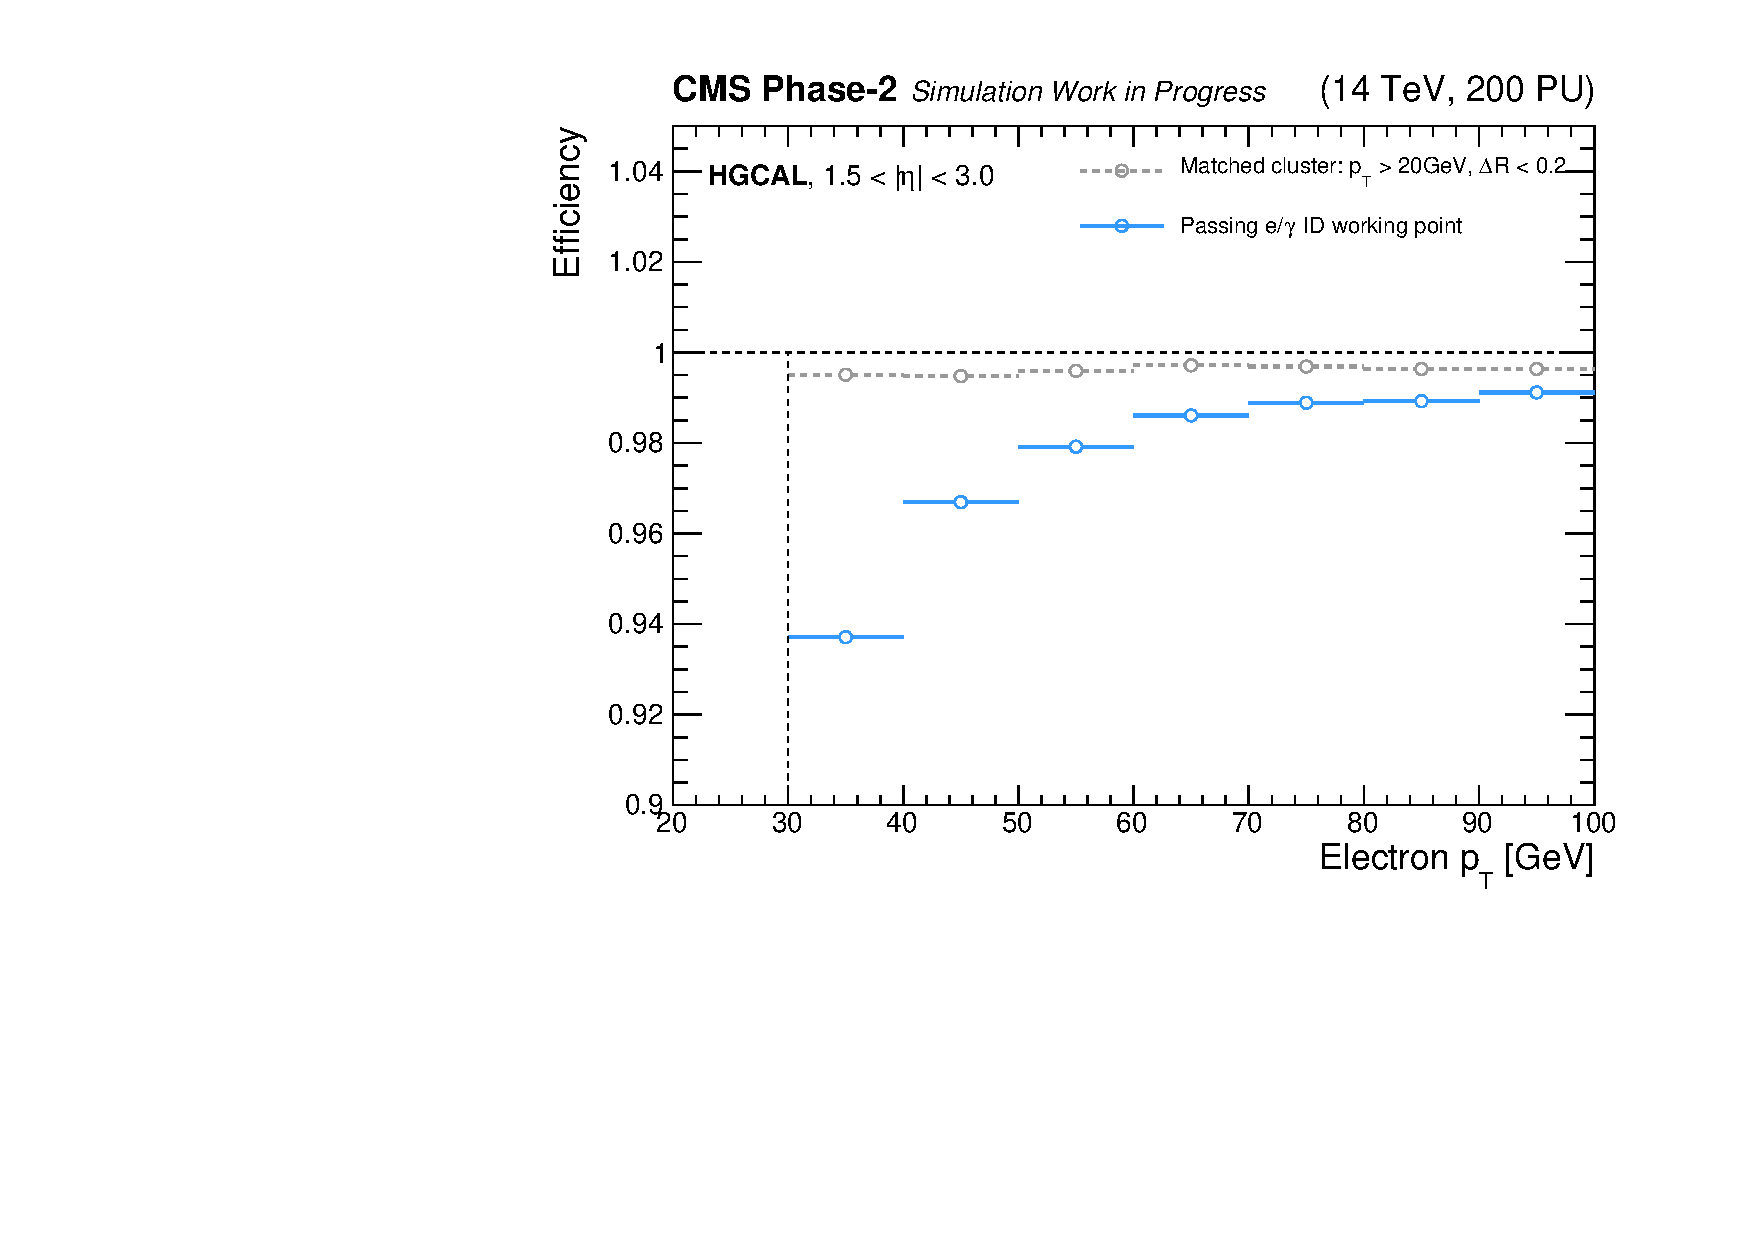
\includegraphics[width=.49\textwidth]{Figures/cms/egid/eff_vs_cl3d_gen_pt.pdf}
  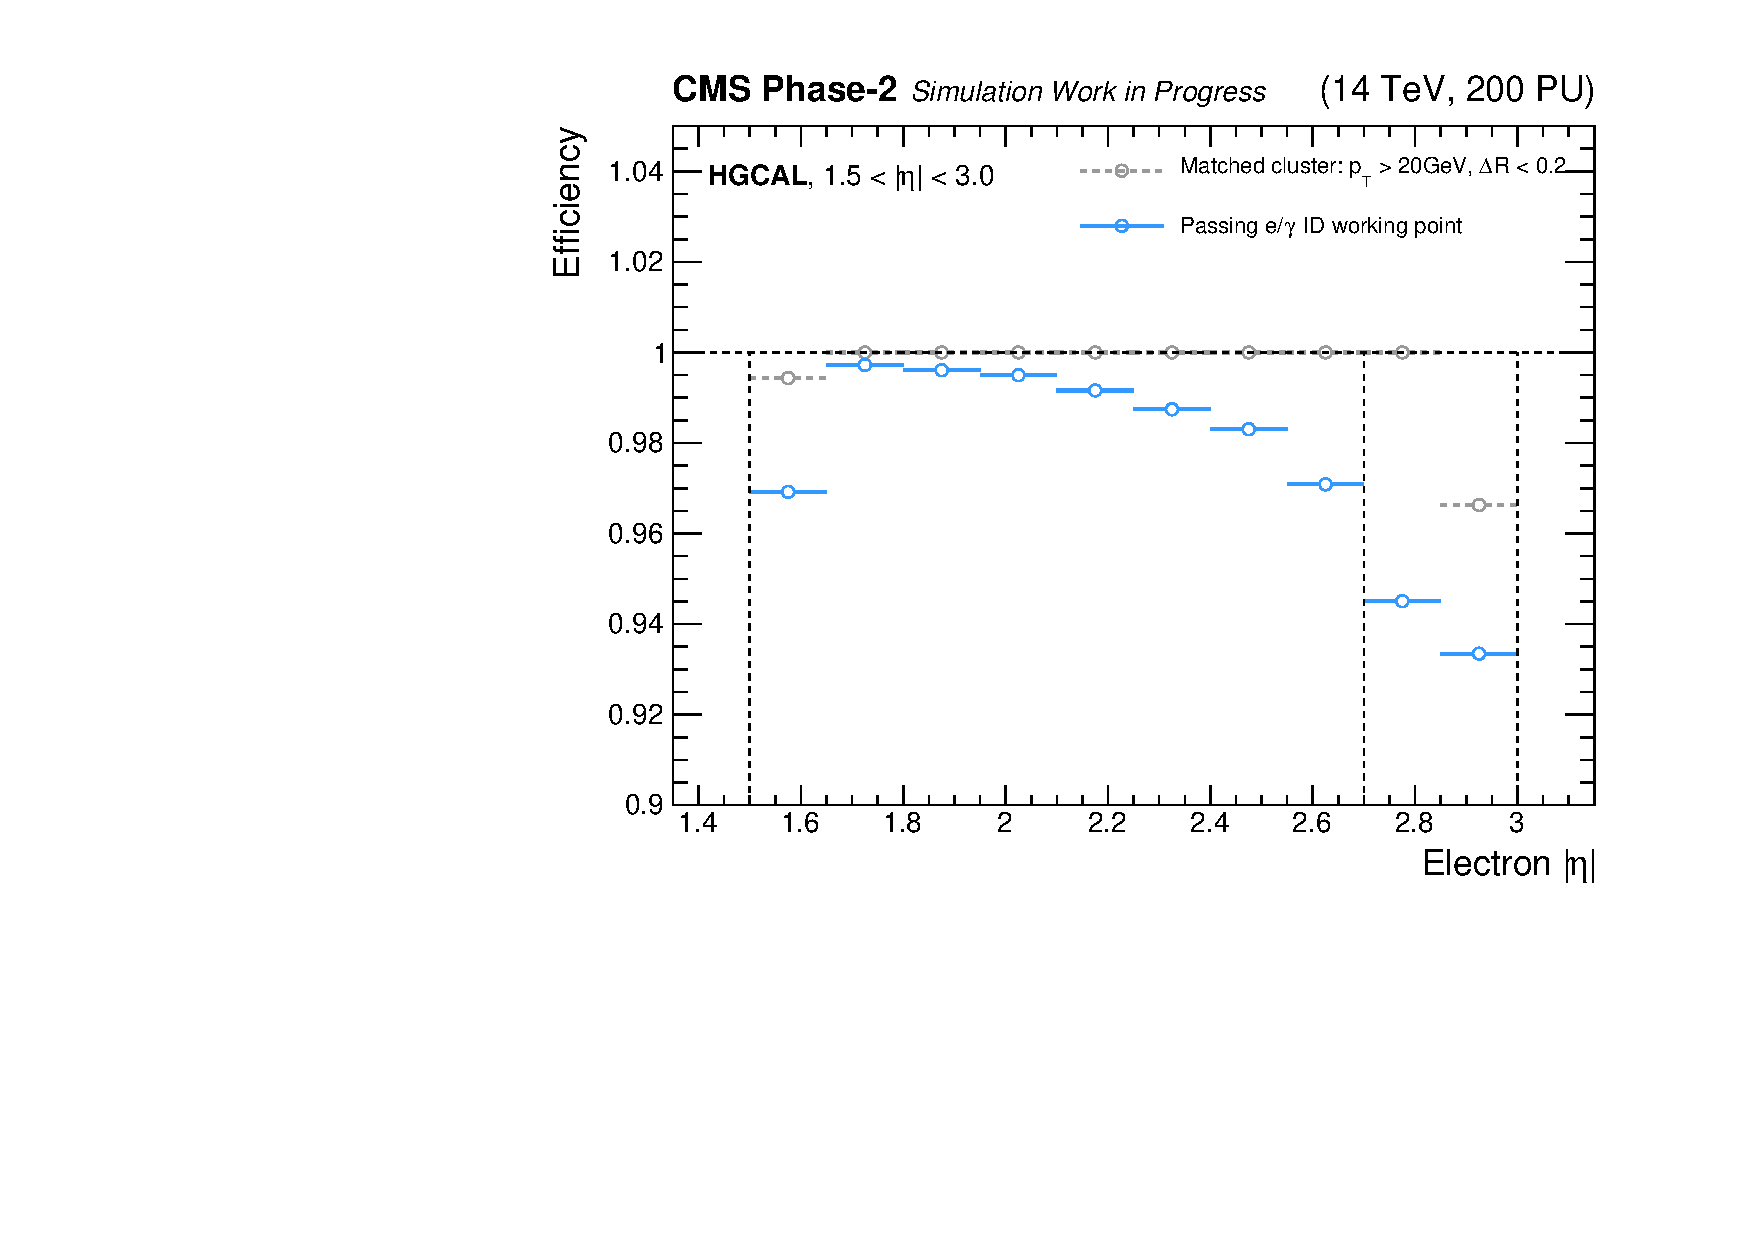
\includegraphics[width=.49\textwidth]{Figures/cms/egid/eff_vs_cl3d_gen_eta.pdf}
  \caption[Efficiency of the $e/\gamma$ identification as a function of electron $p_T$ and $\eta$.]
  {
    Trigger efficiency as a function of the generator level electron $p_T$ (left) and $\eta$ (right). The grey lines indicate the fraction of electrons that contain a matching cluster with reconstructed $p_T>20$~GeV, and $\Delta R<0.2$. The blue lines indicate the fraction of those electrons where the cluster passes the $e/\gamma$ identification working points.
  }
  \label{fig:egid_efficiency}
\end{figure}

Clusters passing the $e/\gamma$ identification BDT working point are subsequently promoted to calorimeter-only $e/\gamma$ candidates. The energy of the candidate is reconstructed and corrected to recover radiative losses from bremsstrahlung. Candidates in the acceptance region of the tracker ($|\eta|<2.4$) are combined with track finder trigger primitives to build track-matched objects for electrons and isolated showers (without a matching track) for photons. The objects then enter the L1T decision process, where an \textit{accept signal} is sent to the detector read-out electronics if the event is deemed to be of interest~\cite{CERN-LHCC-2020-004}.

The BDT algorithm described in this section was developed in offline software. In practice, the L1T operates in real time during data-taking (online) and therefore the algorithm must be implemented in firmware. Recent advances in FPGA technology have enabled the implementation of this particular $e/\gamma$ identification algorithm in firmware, using the \textsc{hls4ml} library~\cite{Duarte_2018}. Crucially, when developing such algorithms it is essential that the resources needed for running are consistent with the design constraints of the Phase-2 L1T. Studies looking at more complex algorithms for the $e/\gamma$ identification, such as neural networks, have been discussed. To be successful, it must be feasible to implement these algorithms in firmware, and the resources needed for running must be compatible with the constraints of the CMS Phase-2 L1T architecture.

\section{Higgs boson physics at the HL-LHC}\label{sec:trilinear}
The HL-LHC offers a wide and diverse physics programme over the coming decades~\cite{Atlas:2019qfx,Bediaga:2018lhg}. In particular, the potential gains from using the HL-LHC dataset for Higgs boson physics are striking~\cite{Cepeda:2019klc}. For example, the combination of future ATLAS and CMS measurements with 3~\abinv of p-p collision data is expected to achieve uncertainties $\mathcal{O}(1.5$--$2.5\%)$ in the Higgs boson couplings to vector bosons, and $\mathcal{O}(2$--$4\%)$ in the Higgs boson couplings to third generation fermions; where the dominant component of the uncertainties in all cases arises from the theoretical prediction. In comparison, the current best measurements from the CMS experiment are $\mathcal{O}(8$--$11\%)$ and $\mathcal{O}(10$--$17\%)$, respectively~\cite{Sirunyan:2020two}. Moreover, the increased dataset will enable more differential measurements, probing increasingly granular regions of the Higgs boson phase space, and will shed light on rarer Higgs boson interactions including the Higgs boson couplings to second generation fermions and the Higgs boson self-coupling. Altogether, the Higgs boson physics programme at the HL-LHC will go a long way towards elucidating the origins of electroweak symmetry breaking.

The analysis described in this section extracts the expected sensitivity of differential $p^H_T$ cross section measurements for Higgs boson production in association with at least one top quark, with the Higgs boson decaying to photons (ttH~+~tH, \Hgg), using the CMS Phase-2 detector at the HL-LHC~\cite{CMS-PAS-FTR-18-020}. It is important to keep in mind that the observation of the ttH production mode was only made in 2018~\cite{Sirunyan:2018hoz,Aaboud:2018urx}. The results presented here show that by the mid-2030s, we will be able to measure this production mode \textit{differentially}, demonstrating impressive sensitivity ($\mathcal{O}(15$--$40\%)$ uncertainties in different $p_T^H$ bins) in a single Higgs boson decay channel. Furthermore, these measurements can be used to indirectly constrain the trilinear Higgs boson self-coupling ($\lambda_3$). Variations in $\kappa_\lambda = \lambda_3/\lambda_3^{\rm{SM}}$ from unity affects the values of the differential cross sections due to NLO corrections in electroweak theory. The expected constraints on $\lambda_3$ from this indirect approach are determined. The analysis uses many of the same techniques as the \Hgg analysis described in chapters~\ref{chap:hgg_overview}--\ref{chap:hgg_results}.

\subsection{Top-associated differential $p_T^H$ cross sections}
Signal and background events are simulated with $\sqrt{s}=14$~TeV using a combination of the \textsc{MG5\_aMC@NLO} (version 2.2.2)~\cite{Alwall:2014hca}, \textsc{Powheg} (version 2.0)~\cite{Nason:2004rx,Frixione:2007vw,Alioli:2008tz,Nason:2009ai,Alioli:2010xd,Hartanto:2015uka}, and \textsc{sherpa} (version 2.2.5)~\cite{Gleisberg:2008ta} generators, interfaced with \textsc{Pythia8} (version 8.205)~\cite{Sjostrand:2014zea} for parton showering and hadronisation. The events are subsequently propagated through the \textsc{delphes} framework~\cite{deFavereau:2013fsa} to perform a \textit{fast simulation} of the CMS Phase-2 detector response under HL-LHC conditions. This works by parametrising the detector efficiency and resolution of the various upgraded Phase-2 subdetectors as a function of the different final-state objects properties (e.g. $p_T$, $\eta$), where the exact form of these parametrisations are derived using detailed simulations~\cite{Contardo:2020886}. The outputs of \textsc{delphes} are then collections of jets, $b$ tagged jets, photons, charged leptons and \met for each generator-level event, which approximately match the expected performance of the CMS Phase-2 detector. All samples are normalised to the expected yields at an integrated luminosity of 3~\abinv.

Events are required to contain two photons with $|\eta^\gamma|<2.5$, excluding the barrel-endcap transition region ($1.44<|\eta^\gamma|<1.57$), with a diphoton invariant mass satisfying $100<m_{\gamma\gamma}<180$~GeV. The leading (sub-leading) photon is also required to have $p^\gamma_T/m_{\gamma\gamma}>1/3$~($1/4$). Additionally, the two photons are required to have an angular separation, $\Delta R_{\gamma\gamma}>0.4$, and each photon must satisfy an isolation requirement which demands the sum of charged particle $p_T$ in a cone of radius $\Delta R_{\gamma}=0.4$, centred on the photon direction, is less than 30\% of the photon $p_T^\gamma$. For events with multiple photon pairs passing this selection, the pair with \mgg closest to the Higgs boson mass are chosen.

Top quarks almost always decay to a W boson and a bottom quark. Therefore, to isolate events consistent with Higgs boson production in association with top quarks, all events are required to contain at least one b tagged jet (see section \ref{sec:hgg_otherobjects}). Events are then separated into two orthogonal global categories depending on the decay products of the W boson: a hadronic global category (W$\rightarrow$qq) and a leptonic global category (W$\rightarrow\ell\nu$). In the hadronic selection, events are required to contain at least three jets, clustered using the anti-$k_T$ algorithm~\cite{Cacciari:2008gp,Cacciari:2011ma} with a distance parameter of $\Delta R=0.4$, where each jet must satisfy $p_T^j>30$~GeV and $|\eta^j|<4$, and be separated by $\Delta R_{j\gamma}>0.4$ with respect to both photon candidates. The leptonic selection requires at least two jets, in addition to at least one isolated muon or electron. The muon or electron must satisfy $p_T^\ell>20$~GeV and $|\eta^\ell|<2.4$, excluding the barrel-endcap transition region for electrons. Muons are required to pass an isolation criteria, such that the sum of all particles $p_T$ in a cone of radius $\Delta R_{\mu}=0.4$, centred on the muon direction, is less than 25\% of the muon $p_T^\mu$. For electrons, the invariant mass of pairs formed from the electron and either photon, $m_{e\gamma}$, is required to be greater than 5~GeV from the Z boson mass to reduce the contamination from \Zee decays. Events passing the leptonic selection are excluded from the hadronic selection to ensure the two categories are orthogonal.

\begin{figure}[htb!]
  \centering
  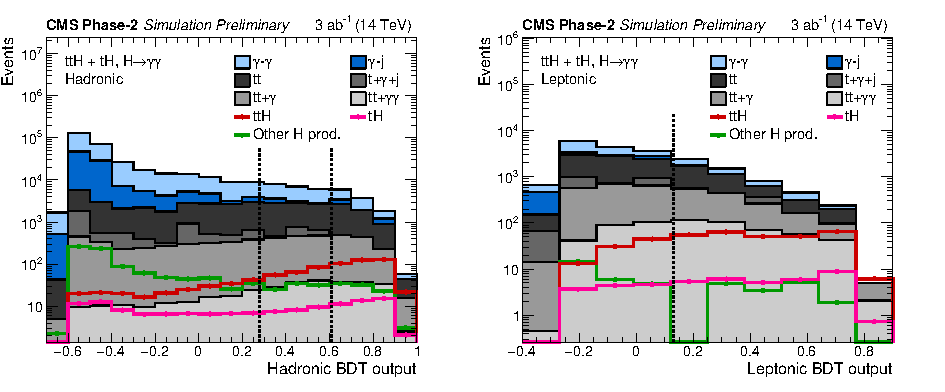
\includegraphics[width=1\textwidth]{Figures/cms/trilinear/CMS-PAS-FTR-18-020_Figure_002.pdf}
  \caption[BDT output score distributions for the HL-LHC sensitivity study]
  {
    The BDT output score distributions for the hadronic (left) and leptonic (right) categories, after the preselection criteria are applied. The background processes are shown by the filled histograms, whilst the Higgs boson production modes are shown by the coloured lines. The dashed vertical lines indicate the positions of the BDT output score thresholds in the event categorisation.
  }
  \label{fig:trilinear_bdt}
\end{figure}

To improve the signal-vs-background discrimination, a BDT is trained independently for each global category using events passing the aforementioned selection criteria. The input features ($\vec{x}$) are the photon, jet and lepton $p_T$ and $\eta$ values, the photon isolation variables, the \met, the scalar sum of all final state objects $p_T$ (mitigating the effects of pileup), the azimuthal separation between the photon pair and the closest jet/leading lepton, and the total number of jets, b tagged jets, and leptons in the event. The BDT output score distributions for the hadronic and leptonic global categories are shown in Figure~\ref{fig:trilinear_bdt}. The plots indicate the important background processes for this study, and also show the contributions from other Higgs boson production modes: ggH + VH. The contamination from VBF production is negligible, and is therefore ignored in this analysis.

Table \ref{tab:trilinear_bins} shows the bin boundaries for which the differential $p_T^H$ cross sections are measured. The hadronic and leptonic global categories are split according to equivalent boundaries in the reconstructed diphoton transverse momentum, $p_T^{\gamma\gamma}$. Events in each $p_T^{\gamma\gamma}$ bin are required to have BDT output score values greater than fixed thresholds\footnote{These thresholds were chosen to maximise the sensitivity to $\kappa_\lambda$.}, shown by the dashed lines in Figure \ref{fig:trilinear_bdt}. In the hadronic channel, the five bins with $p_T^{\gamma\gamma}<350$~GeV are further split into low signal purity and high signal purity regions according to a second threshold on the BDT output score at a value of 0.61. This helps reduce the contamination from ggH production. In total, this corresponds to 17 analysis categories targeting the six $p_T^H$ bins with different requirements on the BDT output scores: 11 for the hadronic channel and six for the leptonic.

\begin{table}[htb]
    \caption[Top-associated differential cross section boundaries]{Bin boundaries for which the differential $p_T^H$ cross sections are measured. To target these bins, the hadronic and leptonic categories are sub-divided by equivalent boundaries on the reconstructed $p_T^{\gamma\gamma}$.}
    \label{tab:trilinear_bins}
    % \vspace{.5cm}
    \centering
    \footnotesize
    \setlength{\tabcolsep}{3pt}
    \renewcommand{\arraystretch}{2}
    \begin{tabular}{p{1cm}<\centering|p{1cm}<\centering|p{1cm}<\centering|p{1cm}<\centering|p{1cm}<\centering|p{1cm}<\centering|p{1cm}<\centering}
        \multicolumn{7}{c}{\textbf{$p_T^H$ or $p_T^{\gamma\gmma}$ bin boundaries [GeV]}} \\ \hline
        0 & 45 & 80 & 120 & 200 & 350 & $\infty$ \\
    \end{tabular}
\end{table}

The cross sections are extracted using a simultaneous maximum likelihood fit to the \mgg distribution in all analysis categories. The signal models are built for each production mode using a sum of Gaussian functions to fit the \mgg peak. In order to account for detector resolution effects, a separate model is constructed for events from each generator-level $p_T^H$ bin in each reconstruction level $p_T^{\gamma\gamma}$ event category. The background models are a set of smoothly falling functions to fit the sum of simulated background events in each event category, where the choice of function is left free to vary in the likelihood fit. This procedure, known as the discrete profiling method~\cite{Dauncey:2014xga}, was previously described in more detail in section \ref{sec:bkg_modeling}. The final signal plus background models are shown for two example analysis categories in Figure~\ref{fig:trilinear_mgg}. The black points, shown purely for illustration purposes, represent a possible HL-LHC dataset and are extracted by throwing random toy data from the signal plus background model. The diphoton mass resolution corresponds to what is expected to be achieved during the HL-LHC operation.

\begin{figure}[htb!]
  \centering
  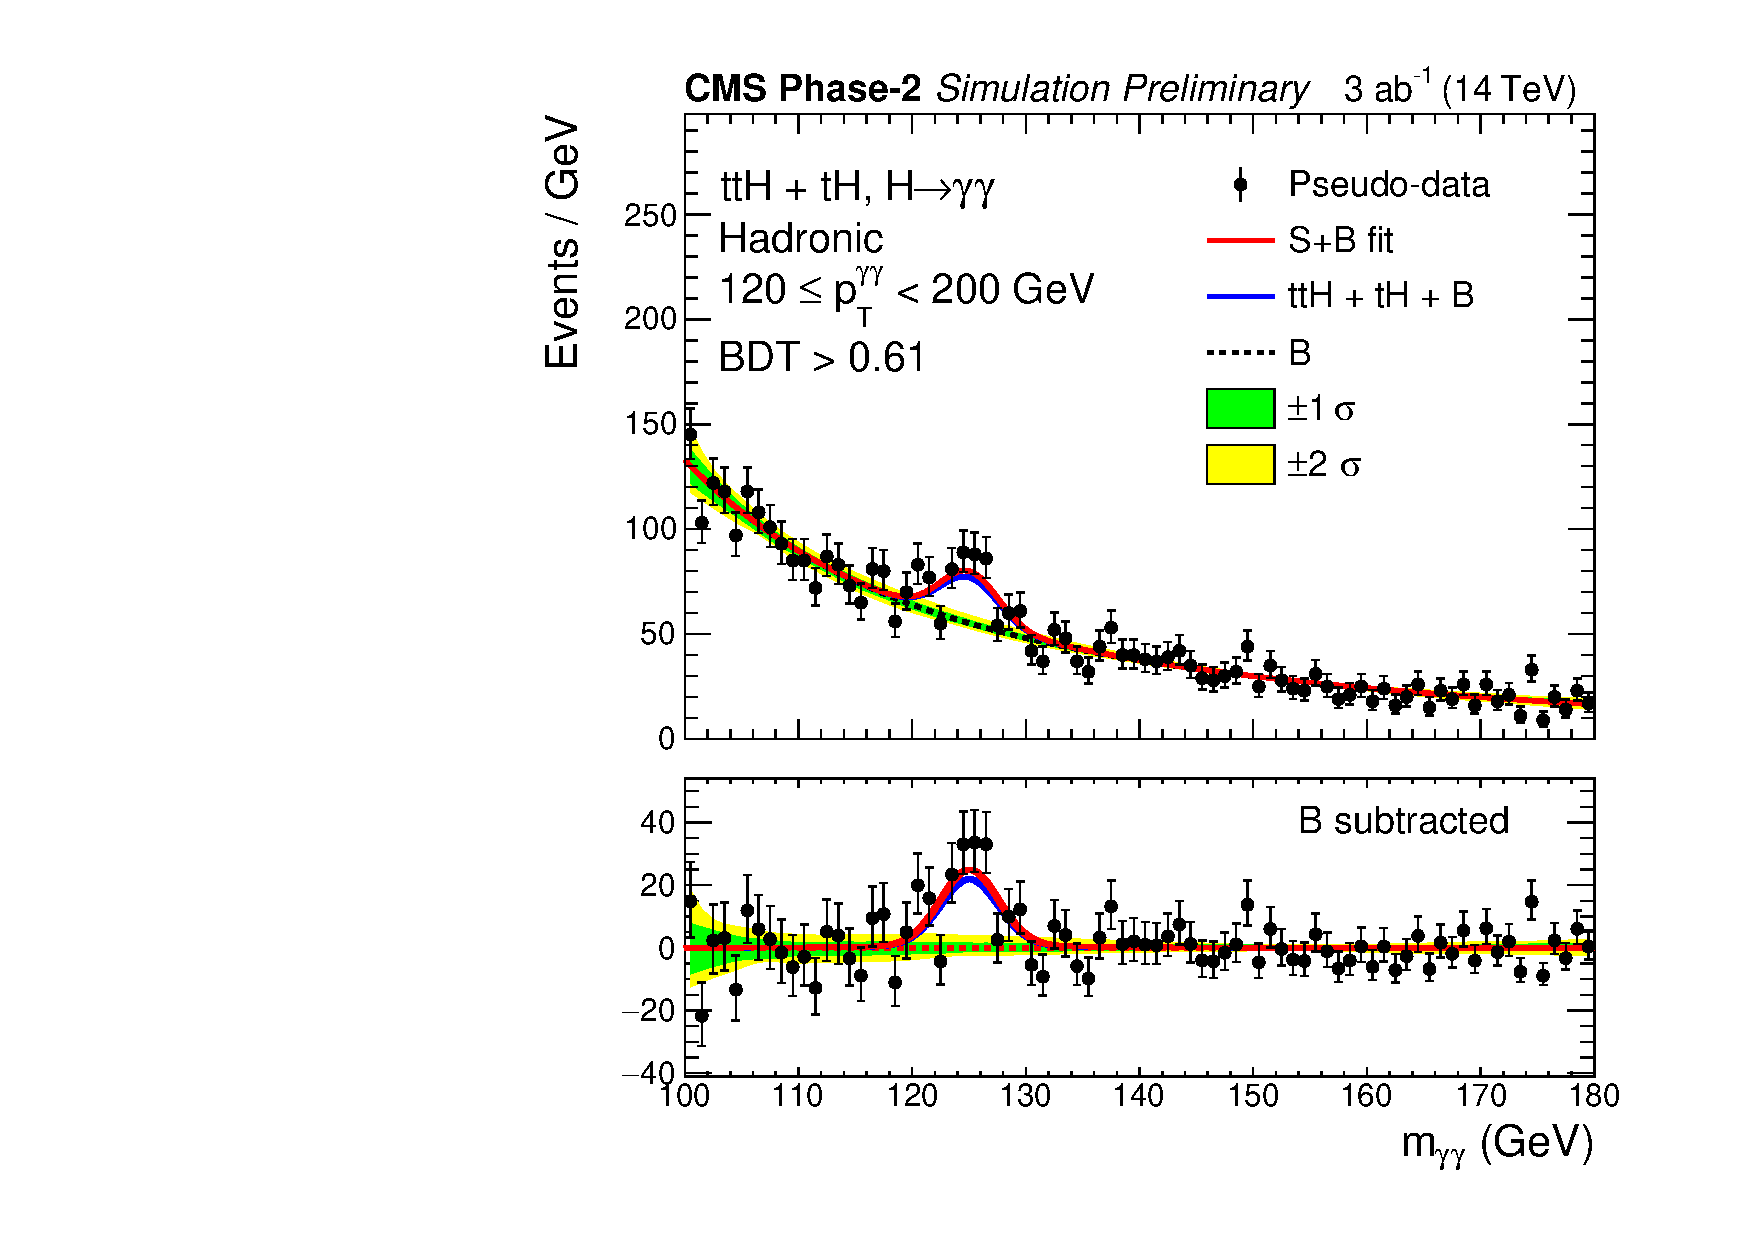
\includegraphics[width=.49\textwidth]{Figures/cms/trilinear/CMS-PAS-FTR-18-020_Figure_004-a.pdf}
  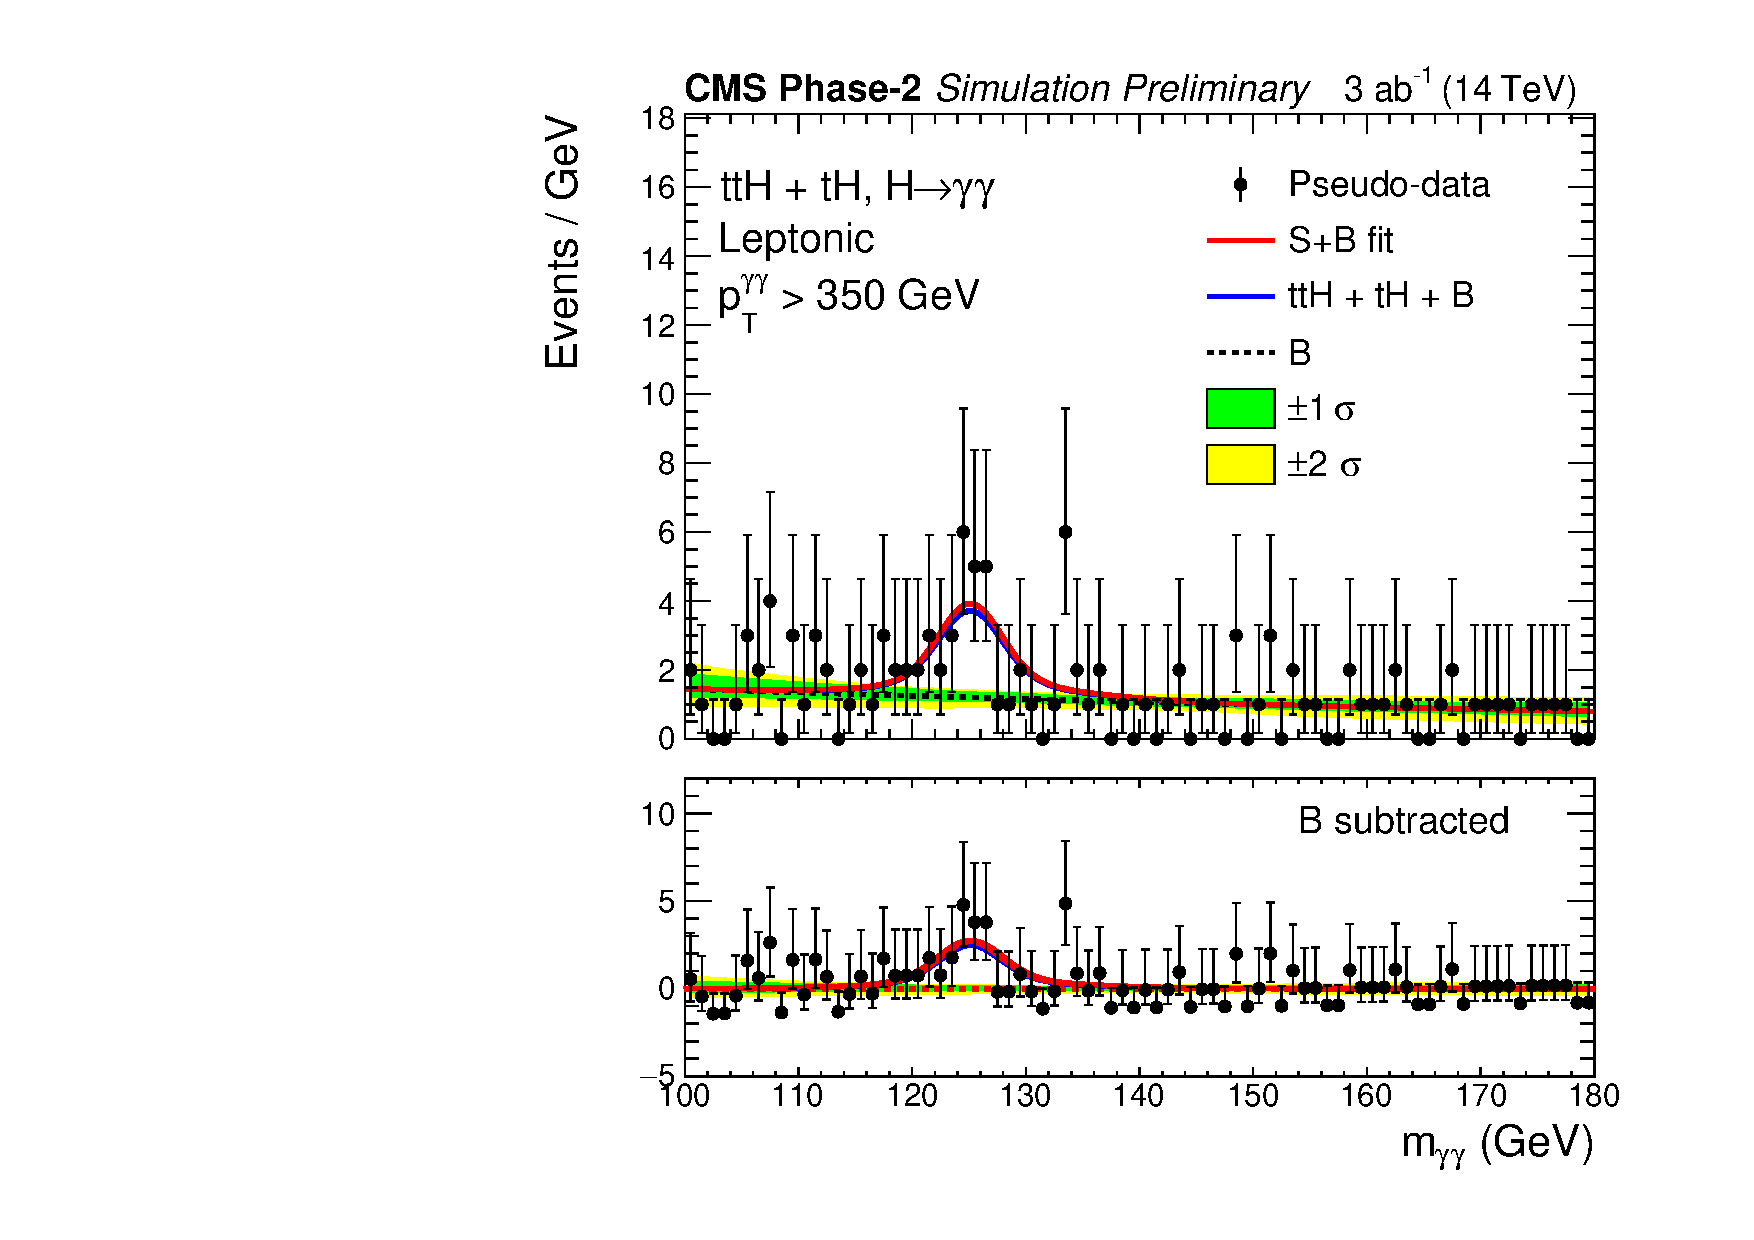
\includegraphics[width=.49\textwidth]{Figures/cms/trilinear/CMS-PAS-FTR-18-020_Figure_005-f.pdf}
  \caption[Diphoton mass distributions for two event categories in the HL-LHC sensitivity study]
  {
     Best-fit signal and background models for the high purity $120<p_T^{\gamma\gamma}<200$~GeV hadronic event category (left) and the $p_T^{\gamma\gamma}>350$~GeV leptonic event category (right). An illustrative pseudo-dataset is thrown from the best-fit models. The one (green) and two (yellow) standard deviation bands show the uncertainties in the background component of the fit. The residuals minus the background component are shown in the lower panels.
  }
  \label{fig:trilinear_mgg}
\end{figure}

A likelihood function is constructed for each analysis category following the procedure introduced in section \ref{sec:category_likelihood}. This uses the corresponding the signal and background models, and an asimov dataset~\cite{Cowan:2010js}. The parameters of interest, $\mu^{i,\gamma\gamma}$, are defined to scale the ttH~+~tH production cross section for each generator-level $p_T^H$ bin, $i$. Defining the parameters in this way enables a likelihood unfolding of the detector resolution effects i.e. the fit accounts for the migrations between the generator-level $p_T^H$ and reconstruction-level $p_T^{\gamma\gamma}$ bins. As this study concerns the expected sensitivity, the asimov dataset corresponds to the SM prediction (all $\mu^{i,\gamma\gamma}=1$). The product over all per-category likelihoods is used to construct a profiled likelihood ratio test-statistic to determine the expected uncertainties in each $\mu^{i,\gamma\gamma}$; a procedure described in detail in section~\ref{sec:results_extraction}.

Systematic uncertainties affecting the signal yield estimates are included as Gaussian constrained nuisance parameters in the likelihood function. Experimental uncertainties originating from the reconstruction and identification efficiencies for photons and b jets, as well as the energy scale and resolution of jets, are modelled as log normal variations in the signal yields. Theoretical uncertainties which cause the migration of signal events between event categories are accounted for. Additionally, theoretical uncertainties which modify the overall rates of ggH and VH production are included, as these production modes are not explicitly extracted in the fit. Parameters of the background model functions are free to vary in the fit, and are therefore constrained directly from data. This means the uncertainties in the background estimation are statistical in nature.

The $\mu^{i,\gamma\gamma}$ parameters and their uncertainties are converted to fiducial cross sections times branching ratio, $\sigma^{\rm{ttH+tH}}_{\rm{fid}}\cdot\mathcal{B}^{\gamma\gamma}$, by correcting for the event selection efficiencies. The fiducial region is common to both the hadronic and leptonic selections, and is defined according to the generator-level events as follows:
\begin{itemize}
    \item Higgs boson rapidity: $|Y_H|<2.5$.
    \item Two photons from the Higgs boson decay: $p_T^\gamma > 20$~GeV and $|\eta^\gamma|<2.5$.
    \item At least two jets: $p_T^\gamma > 25$~GeV and $|\eta^j|<4$.
    \item At least one of the jets, satisfying the above criteria, originates from a b quark.
\end{itemize}
\noindent
A small fraction of the events passing the full selection (0.7\% in the hadronic selection, and 0.4\% in the leptonic selection) are not contained in the fiducial region. Although these events are included in the construction of the likelihood, they are subtracted when calculating the fiducial cross sections.

Figure \ref{fig:trilinear_dxs} shows the expected differential fiducial cross sections times branching ratio, for Higgs boson production in association with at least one top quark, in bins of $p_T^H$. The error bars indicate the combined statistical and systematic uncertainties in the measurements using 3~\abinv of HL-LHC data. Analogous likelihood fits are performed using only the hadronic event categories and only the leptonic event categories, shown by the red and purple error bars, respectively. In general, the hadronic channel is observed to provide greater sensitivity. This is a result of the larger absolute signal yield after selection, compared to the leptonic channel. The theoretical uncertainties in the predicted ttH~+~tH cross sections, displayed by the yellow boxes in the plot, are calculated by modifying the renormalisation and factorisation scales up and down by a factor of 2.

\begin{figure}[htb!]
  \centering
  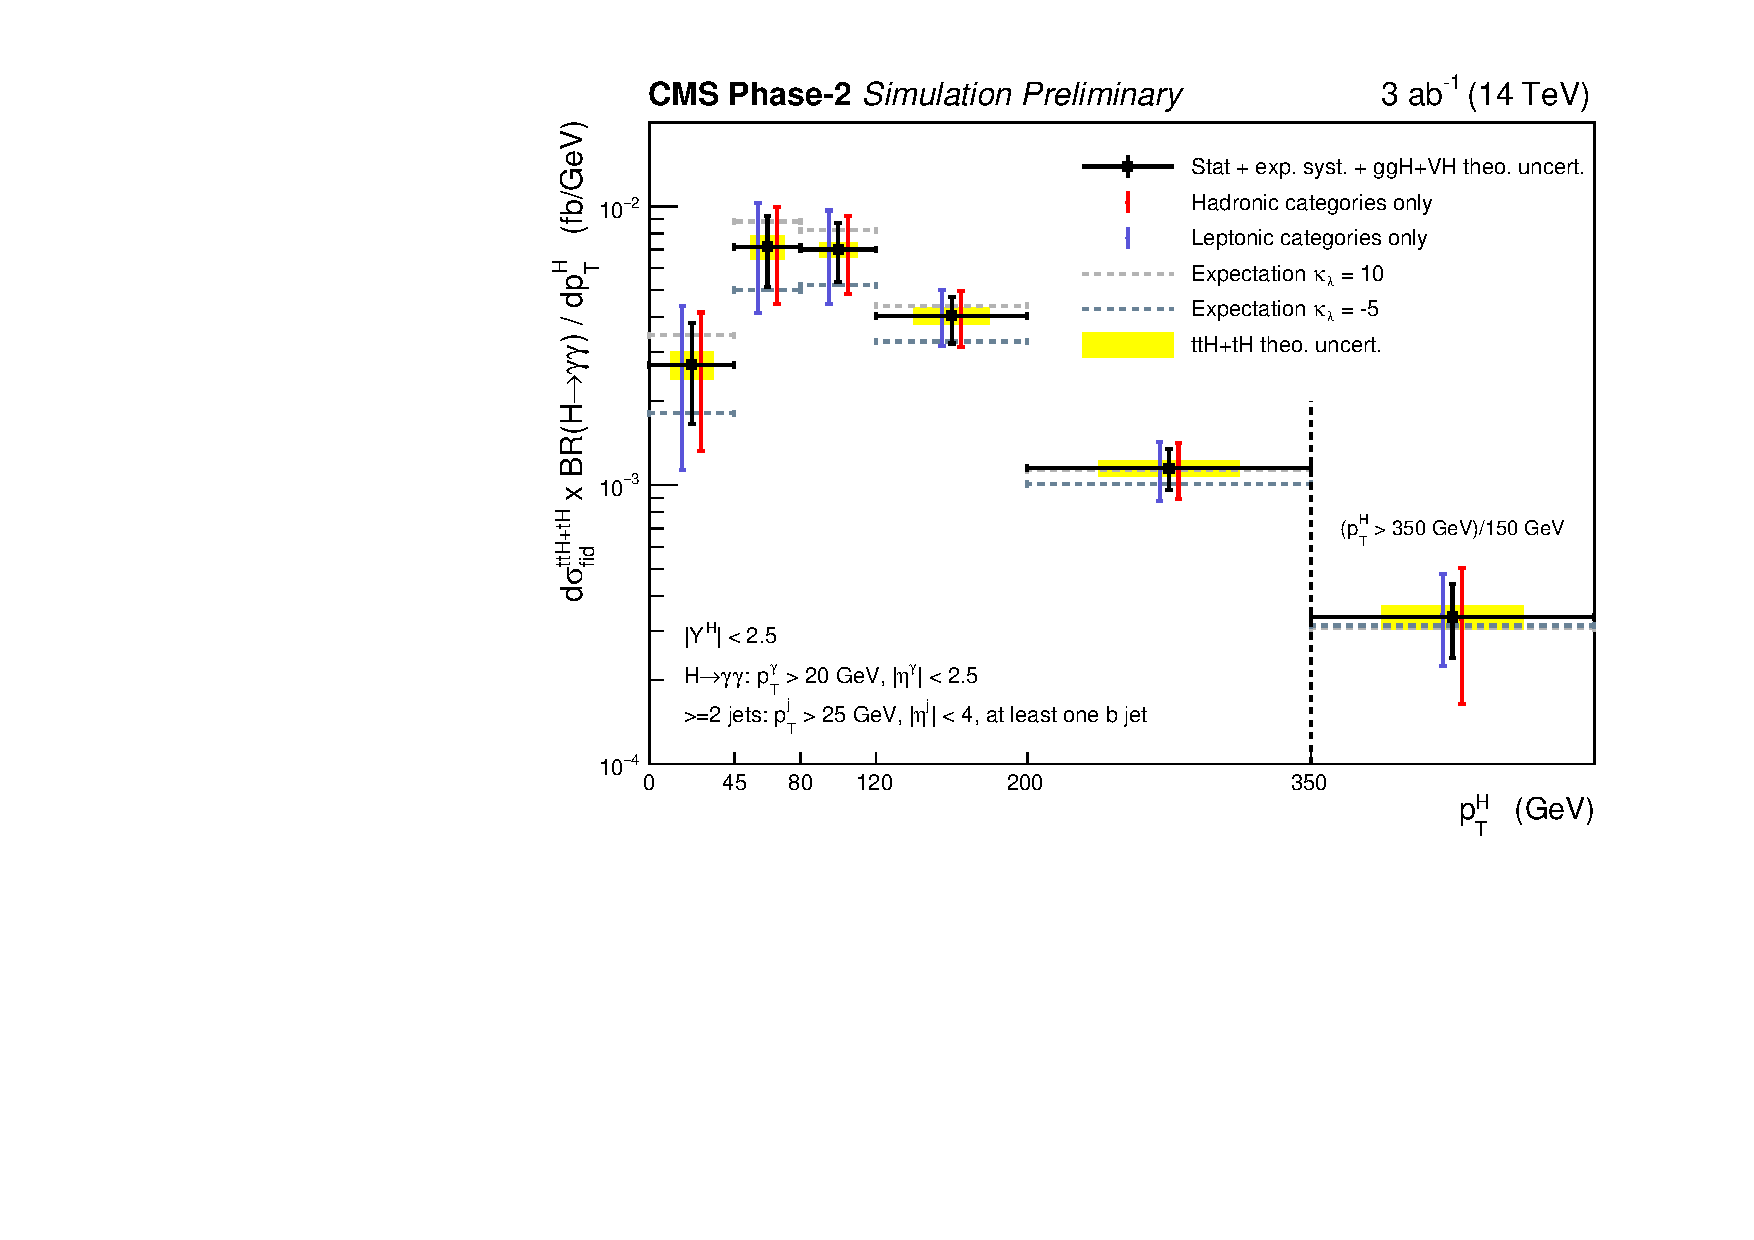
\includegraphics[width=.8\textwidth]{Figures/cms/trilinear/CMS-PAS-FTR-18-020_Figure_006.pdf}
  \caption[Expected top-associated differential $p_T^H$ cross section measurements at the HL-LHC]
  {
    Expected ttH~+~tH differential cross sections times branching ratio, in bins of $p_T^H$, for 3~\abinv of HL-LHC data. These are for the fiducial region of phase space defined in the bottom left of the plot. The error bars include the statistical, experimental systematic and ggH + VH theoretical systematic uncertainties. The theoretical uncertainties on the ttH~+~tH cross section predictions, originating from the uncertainty in the renormalisaion and factorisation scales, are shown by the shaded yellow boxes. The sensitivities extracted from the hadronic and leptonic categories alone, are indicated by the red and purple error bars respectively. The cross section for the $p_T^H=[350,\infty]$~GeV bin is scaled by the width of the previous bin. Additionally, the expected cross sections for anomalous values of the Higgs boson self-coupling ($\kappa_\lambda=10$ and $\kappa_\lambda=-5$) are shown by the horizontal dashed lines.
  }
  \label{fig:trilinear_dxs}
\end{figure}

The expected sensitivities are summarised in table~\ref{tab:trilinear_dxs_results}. Many extensions to the SM predict modifications to the Higgs boson interaction with the top quark. By measuring the differential cross sections within uncertainties $\mathcal{O}$(15--40\%), and therefore gaining a handle on the kinematic spectrum of top-associated production, we will be able to tightly constrain potential new physics affecting the top-Higgs sector. One such example concerning anomalous values of the Higgs boson self coupling, $\lambda_3$, is provided below.

\begin{table}[htb!]
  \centering
%   \footnotesize
  \renewcommand{\arraystretch}{1.8}
  \setlength{\tabcolsep}{15pt}
  \caption[Expected sensitivities of top-associated differential cross sections at the HL-LHC]
  {
    Expected uncertainties in the ttH~+~tH differential $p_T^H$ fiducial cross sections times branching ratio for 3~\abinv of data collected at the HL-LHC. The uncertainty is decomposed into the statistical and systematic components.
  }
  \label{tab:trilinear_dxs_results}
  \hspace*{-1cm}
  \begin{tabular}{c|ccc}
  \hline
  \multirow{2}{*}{$p_T^H$ bin} & \multicolumn{3}{c}{Expected $\pm1\sigma$ uncertainties} \\ 
  & Total & Stat unc. & Syst unc. \\ \hline 
  $[0,45]$  & $^{+41\%}_{-39\%}$ & $^{+41\%}_{-39\%}$ & $^{+4\%}_{-2\%}$ \\
  $[45,80]$  & $^{+29\%}_{-28\%}$ & $^{+29\%}_{-28\%}$ & $^{+3\%}_{-2\%}$ \\
  $[80,120]$  & $^{+24\%}_{-24\%}$ & $^{+24\%}_{-24\%}$ & $^{+3\%}_{-2\%}$ \\
  $[120,200]$  & $^{+17\%}_{-21\%}$ & $^{+16\%}_{-20\%}$ & $^{+3\%}_{-3\%}$ \\
  $[200,350]$  & $^{+17\%}_{-17\%}$ & $^{+16\%}_{-16\%}$ & $^{+5\%}_{-5\%}$ \\
  $[350,\infty]$  & $^{+33\%}_{-30\%}$ & $^{+30\%}_{-28\%}$ & $^{+14\%}_{-13\%}$ \\
  \hline
\end{tabular}
  \hspace*{-1cm}
\end{table}

\subsection{Constraining $\kappa_\lambda$}
Measurements of the trilinear self-interaction of the Higgs boson are of upmost priority in future physics programmes~\cite{Cepeda:2019klc}; they provide constraints on the shape of the Higgs potential close to the minimum, and will shed light on the dynamics of EWSB, including the order of the electroweak phase transition~\cite{PhysRevD.13.974,PhysRevD.20.2619,Kajantie:1995kf,Csikor:1998eu}. In the SM, the trilinear coupling strength, $\lambda^{\rm{SM}}_3=m_H^2/2v$, is fixed according to the Higgs boson mass, $m_H$, and the vacuum expectation value, $v$. BSM physics, such as an extended scalar sector, can modify the value of $\lambda_3$ without affecting $m_H$ and $v$.

The direct approach to constraining $\lambda_3$ is via searches for di-Higgs production (HH), which depends on $\lambda_3$ at LO. A number of HH final states have been explored by ATLAS and CMS at $\sqrt{s}=13$~TeV~\cite{Sirunyan:2018ayu,Aad:2019uzh}. The current best constraints on $\lambda_3$ come from the full Run 2 CMS HH$\rightarrow$bb$\gamma\gamma$ analysis~\cite{Sirunyan:2020xok}, which excludes $\kappa_\lambda=\lambda_3/\lambda_3^{\rm{SM}}$ values outside of the range $-3.3 < \kappa_\lambda < 8.5$ at the 95\% confidence level. Despite this impressive result, HH production is not expected to be observed at $5\sigma$ until after the HL-LHC operation~\cite{Cepeda:2019klc}. This is due to the small SM cross section ($31.1^{+1.4}_{-2.0}$~fb at $\sqrt{s}=13$~TeV), which suffers from destructive interference amongst diagrams~\cite{Grazzini:2018bsd}. Consequently, alternative strategies for probing $\lambda_3$ are in high demand.

One such approach is to exploit radiative corrections to inclusive and differential single-Higgs boson production rates~\cite{Degrassi:2016wml,Maltoni:2017ims,Gorbahn:2016uoy,Bizon:2016wgr,DiVita:2017eyz}. At NLO in electroweak theory, single-Higgs boson production includes diagrams with the trilinear self-interaction, such as that shown in Figure~\ref{fig:trilinear_feynman}. The effects of a modified $\lambda_3$ are sizeable for Higgs boson production in association with top quarks (ttH and tH) or a vector boson (VH). This is due to the large mass of the associated particles providing a larger coupling to the virtual Higgs boson. Moreover, the deformations to the Higgs boson rates are shown to have a non-flat kinematic dependence on $\lambda_3$~\cite{Maltoni:2017ims,DiVita:2017eyz}. As a result, differential cross section measurements can disentangle the effects of a modified $\lambda_3$ from other effects such as the presence of an anomalous top-Higgs coupling. Altogether, these features mean the ttH~+~tH differential cross section measurements introduced in the previous section provide an excellent candidate for indirectly probing $\lambda_3$.

\begin{figure}[htb!]
  \centering
  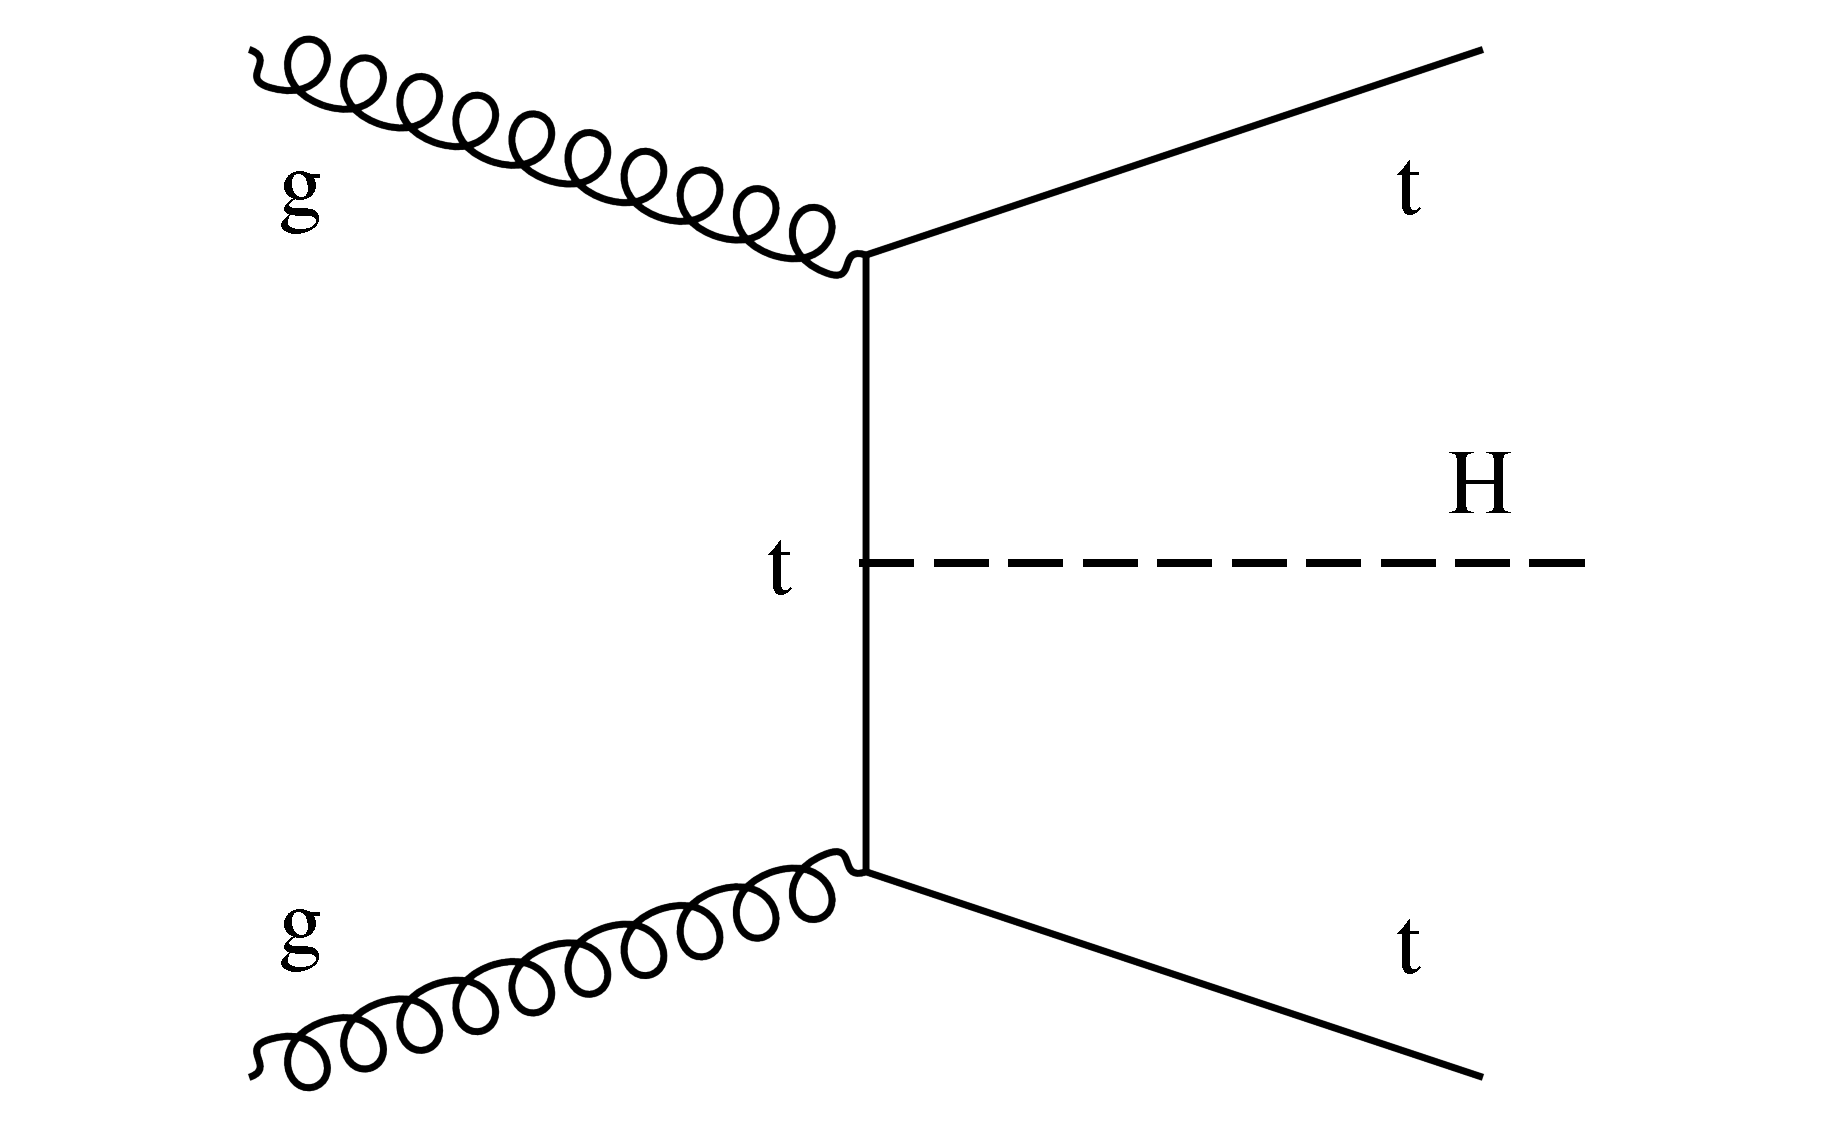
\includegraphics[width=.35\textwidth]{Figures/cms/trilinear/CMS-PAS-HIG-19-005_Figure_001-d.pdf}
  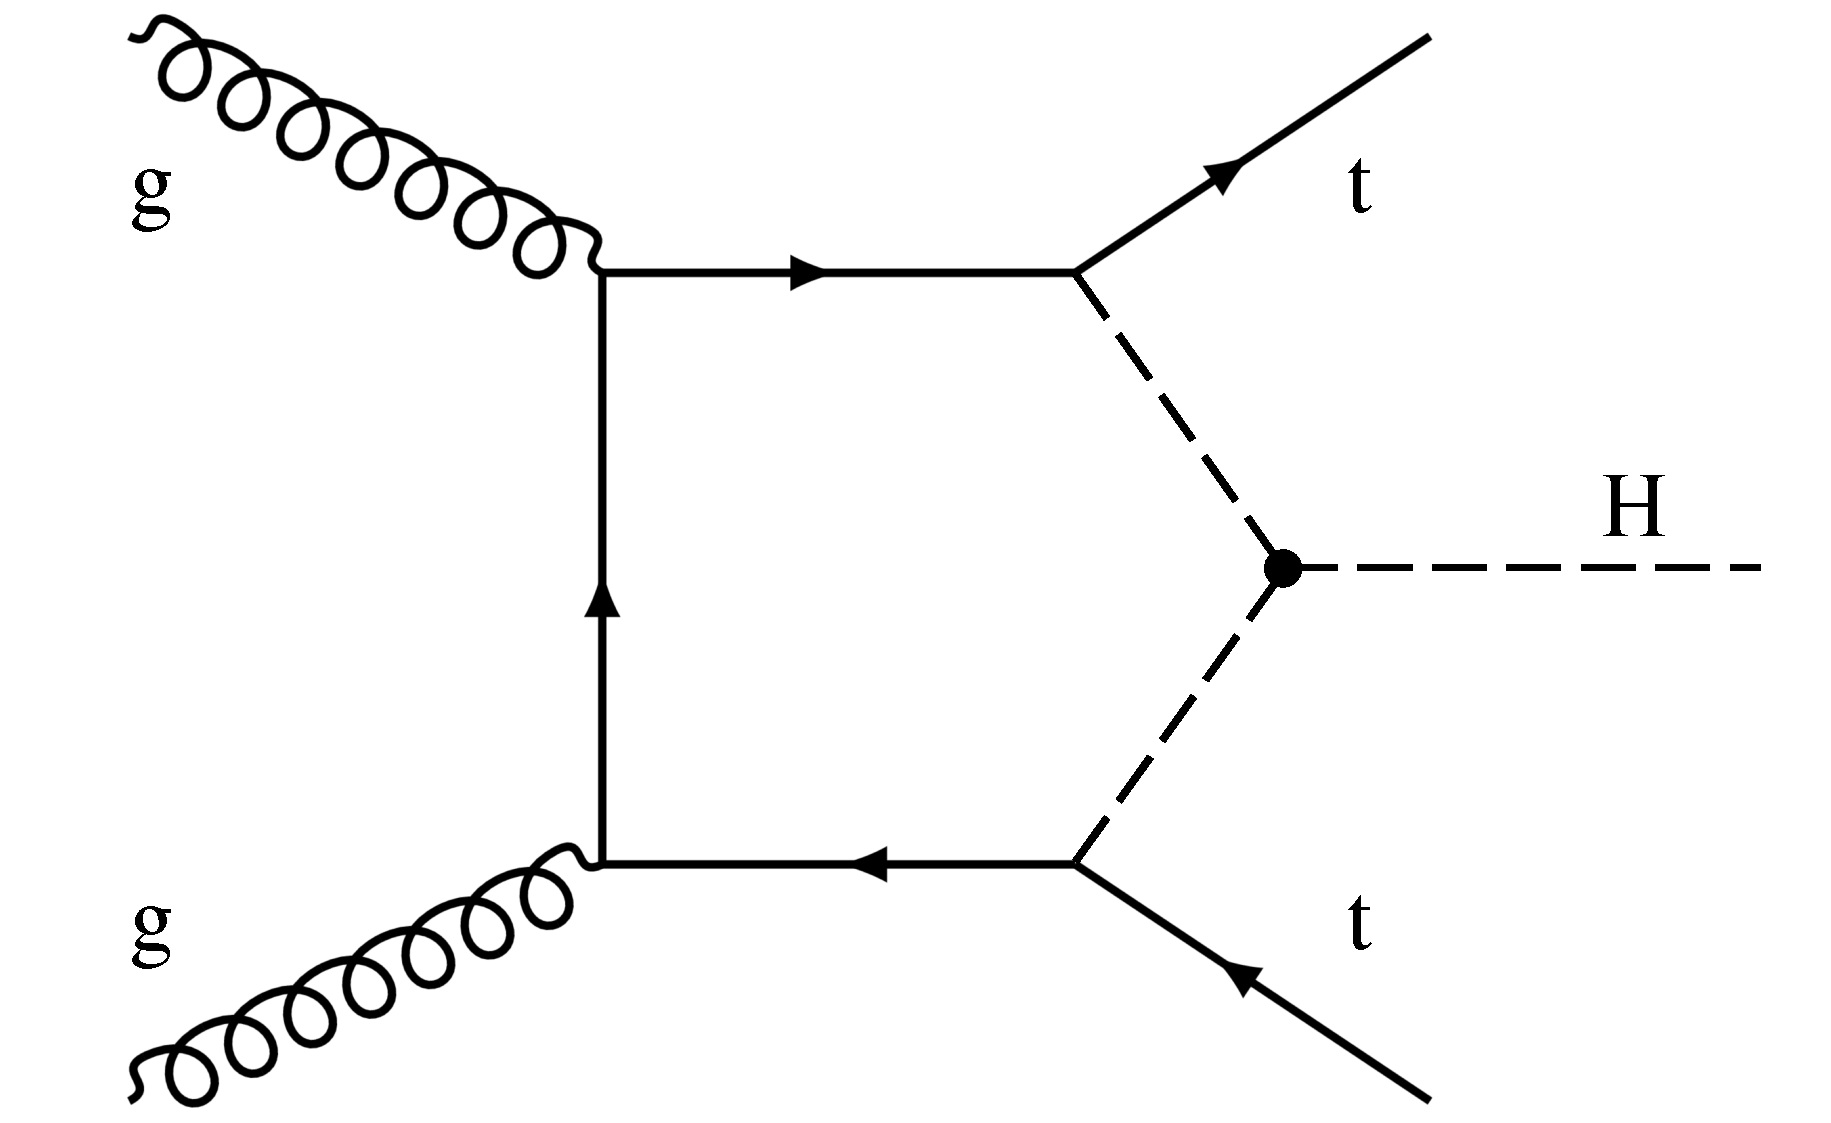
\includegraphics[width=.35\textwidth]{Figures/cms/trilinear/CMS-PAS-FTR-18-020_Figure_001.pdf}
  \caption[Feynam diagram showing a $\lambda_3$-dependent NLO correction to ttH production.]
  {
    Feynamn diagrams for ttH production at LO (left) and a $\lambda_3$-dependent correction at NLO (right).
  }
  \label{fig:trilinear_feynman}
\end{figure}

The effect of anomalous $\kappa_\lambda=\lambda_3/\lambda_3^{\rm{SM}}$ values on the single-Higgs boson production cross sections and decay widths have been predicted~\cite{Maltoni:2017ims}. The cross section is parametrised as a function of $\kappa_\lambda$ according to the following function,
\begin{equation}\label{eq:trilinear_scaling}
    \mu(\kappa_\lambda,C_1) = \frac{\sigma}{\sigma_{\rm{SM}}} = \frac{1+\kappa_\lambda C_1 + \delta Z_H}{(1-(\kappa_\lambda^2-1)\delta Z_H)(1+C_1+\delta Z_H)}.
\end{equation}
The $\delta Z_H=-1.536\times10^{\rm{-3}}$ component originates from the Higgs boson wave function renormalisation and is universal to all production modes. The $C_1$ parameter is defined as the interference between the LO Born matrix element, $\mathcal{M}^{\rm{LO}}$, and the virtual $\lambda_3$-dependent SM matrix element at one-loop, $\mathcal{M}^{\rm{NLO}}_{\lambda_3^{\rm{SM}}}$, 
\begin{equation}
    C_1(\{p\}) = \frac{2{\rm{Re}}(\mathcal{M}^{{\rm{LO}}*}\mathcal{M}^{\rm{NLO}}_{\lambda_3^{\rm{SM}}})}{|\mathcal{M}^{{\rm{LO}}}|^2}.
\end{equation}
\noindent
Crucially, $C_1$, depends both on the Higgs boson production mode, and on some final state observable, $p$. The $C_1$ factors relevant for this analysis are derived using the electroweak reweighting tool described in Ref.~\cite{EWreweightingtool}. Leading order (LO) parton-level ttH, tH and VH events are simulated using the \textsc{MG5\_aMC@NLO} (version 2.5.5) generator~\cite{Alwall:2014hca}. The tool then calculates $\lambda_3$-dependent corrections at NLO ($\mathcal{O}(\lambda_3)$) by reweighting events on an event-by-event basis. A diagram filter is applied to select only the relevant one-loop matrix elements which feature the trilinear coupling. The $C_1$ factors are then extracted by taking the ratio of the $\mathcal{O}(\lambda_3)$ to LO contributions in bins of the generator-level $p_T^H$ spectrum. These $C_1$ factors are plugged into equation~\ref{eq:trilinear_scaling} to determine the differential cross section scaling functions. It should be noted that this parametrisation relies on the assumption that higher-order QCD effects and other NLO EW contributions factorise from the anomalous $\lambda_3$ effects. The validity of this assumption has been studied in detail in Ref.~\cite{Maltoni:2017ims}.

The reweighting tool does not accommodate ggH production, due to the presence of the ggH loop at LO. For this reason, an inclusive scaling function is used for ggH production, where the value of $C_1=0.0066$ is taken directly from Ref.~\cite{Degrassi:2016wml}; this is small compared to the $C_1$ values for the ttH and tH production modes. Additionally, there is a small correction to the \Hgg decay rate from anomalous $\kappa_\lambda$ values which is also taken from Ref.~\cite{Degrassi:2016wml}. The final scaling functions, $\mu^{i,\gamma\gamma}(\kappa_\lambda)$, for each Higgs boson production mode, split into the different generator-level $p_T^H$ bins, are shown in Figure~\ref{fig:trilinear_sf}.

\begin{figure}[htb!]
  \centering
  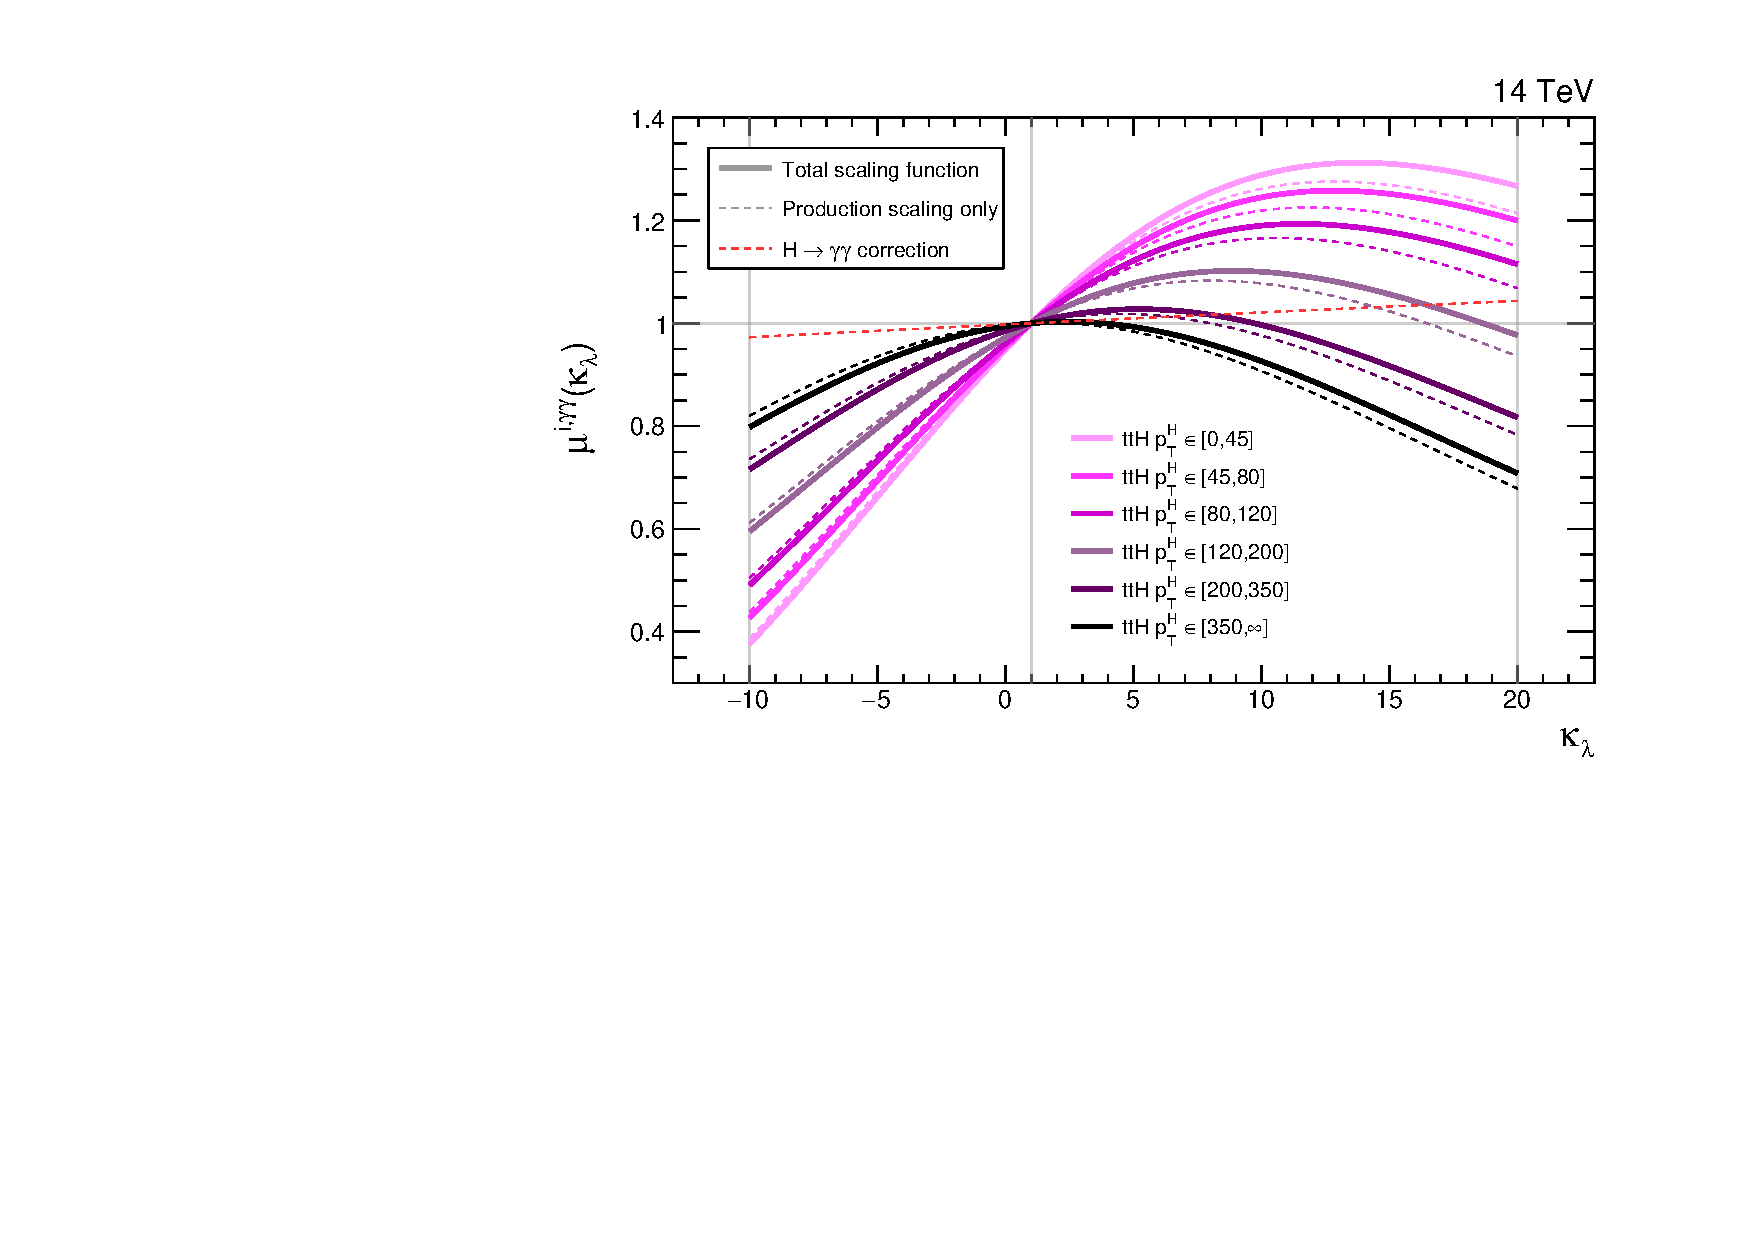
\includegraphics[width=.49\textwidth]{Figures/cms/trilinear/ttH.pdf}
  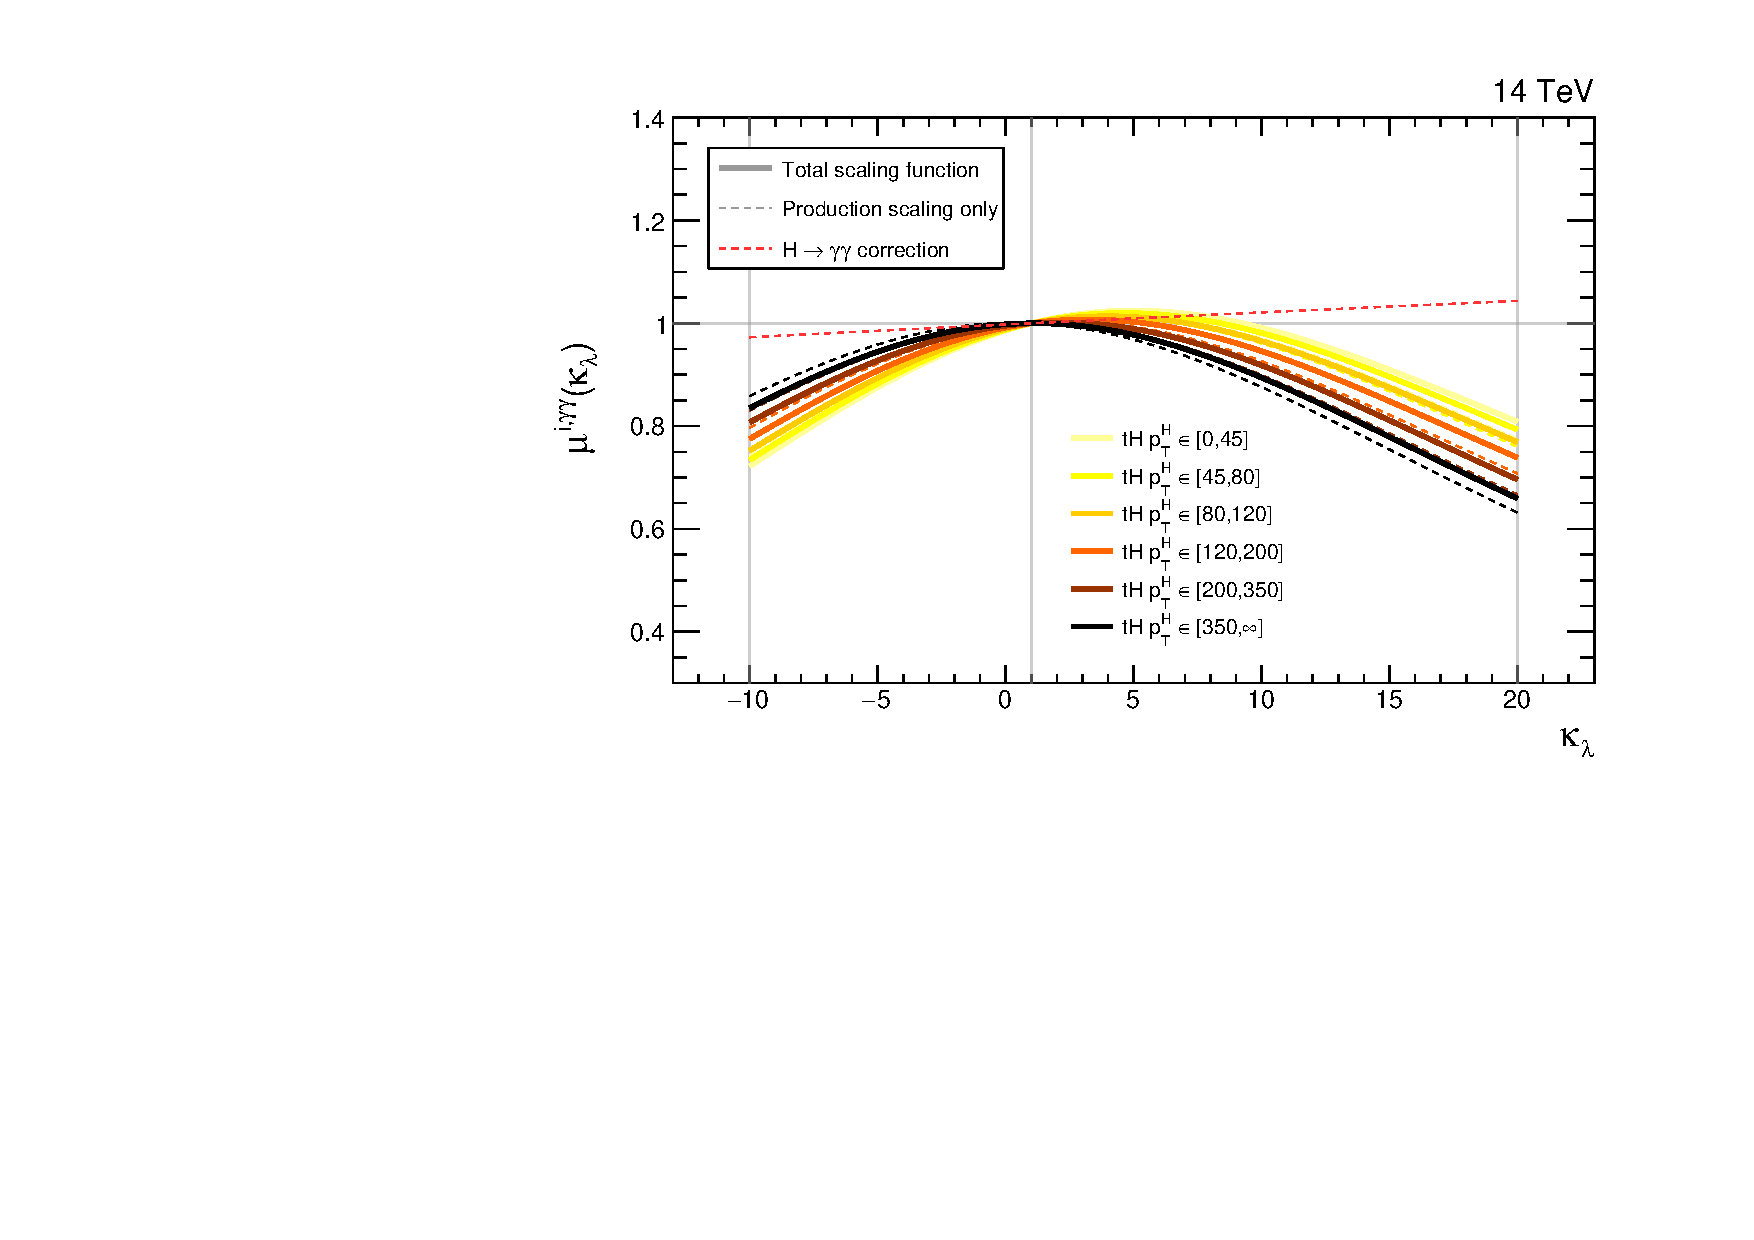
\includegraphics[width=.49\textwidth]{Figures/cms/trilinear/tH.pdf}
  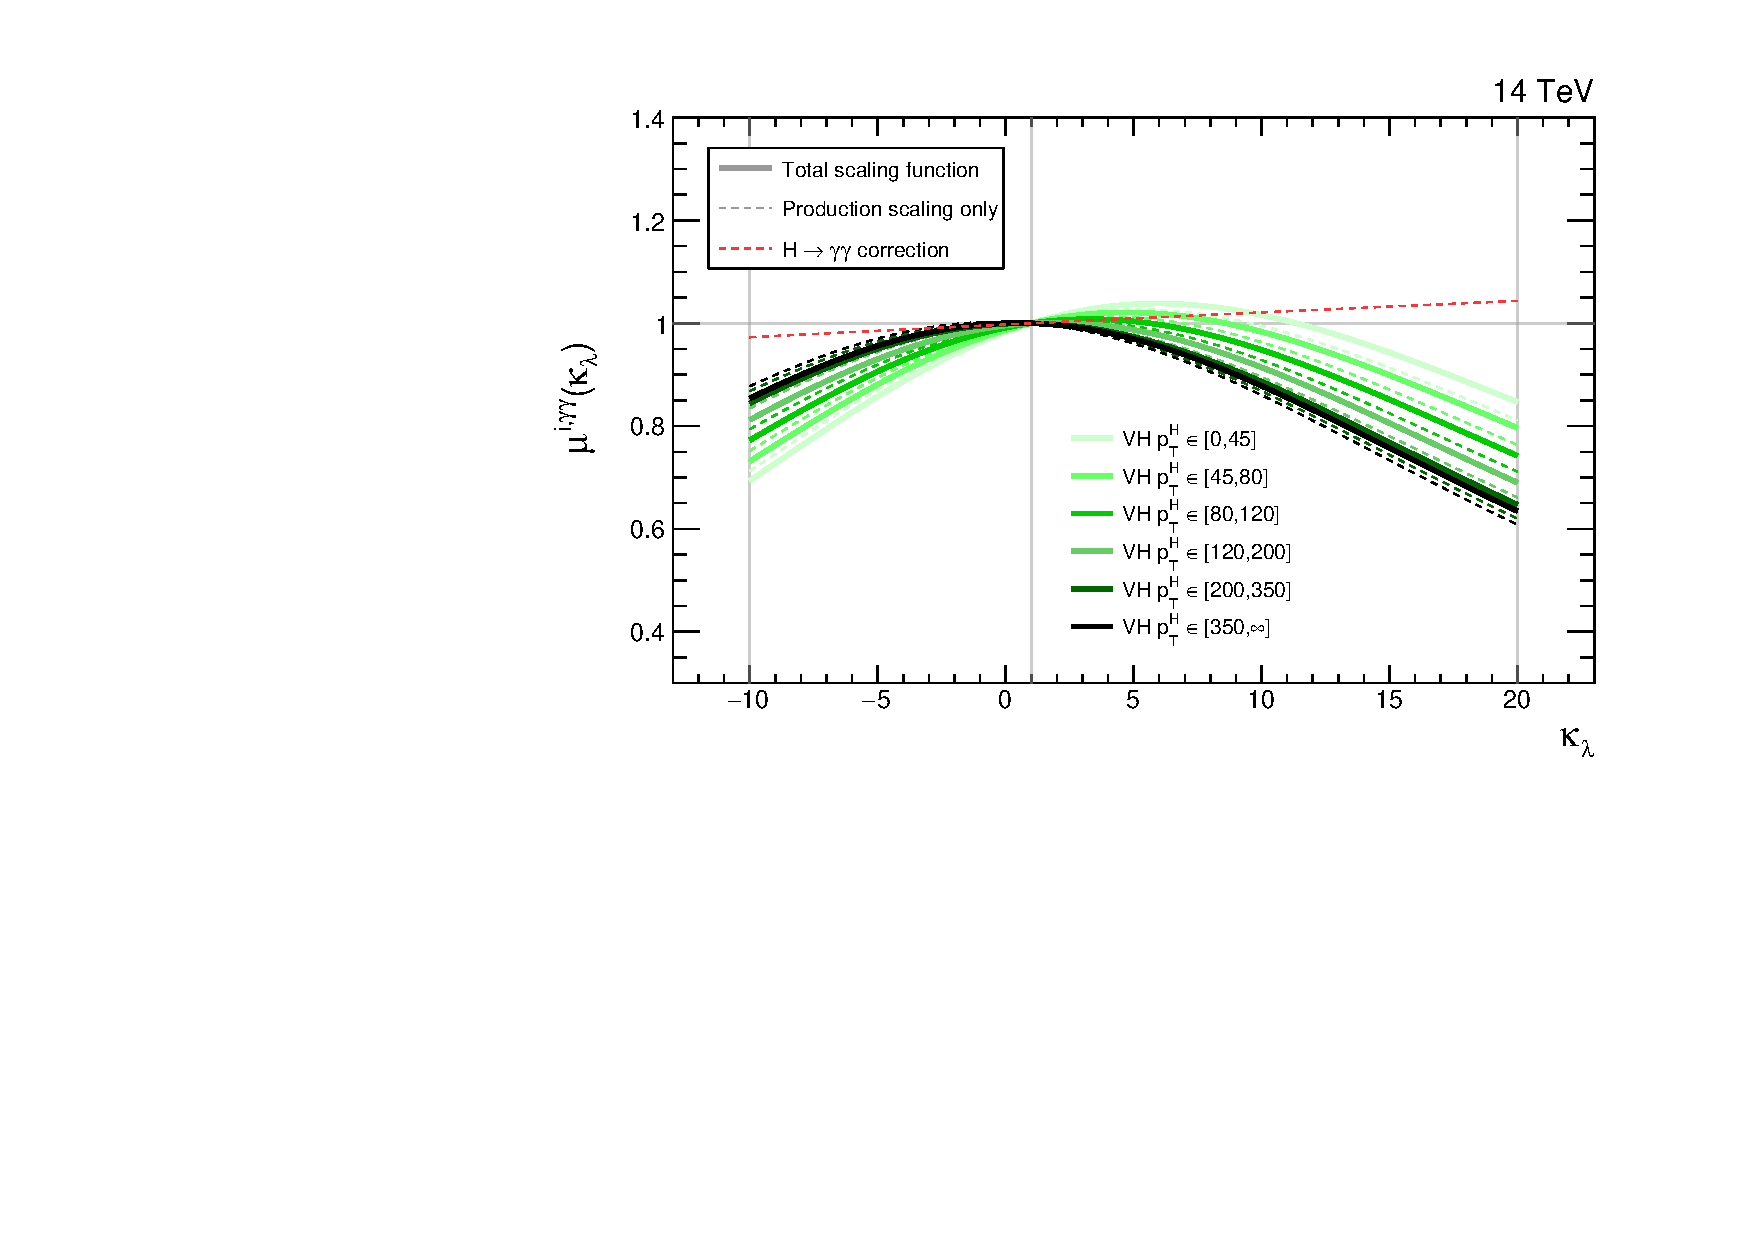
\includegraphics[width=.49\textwidth]{Figures/cms/trilinear/VH.pdf}
  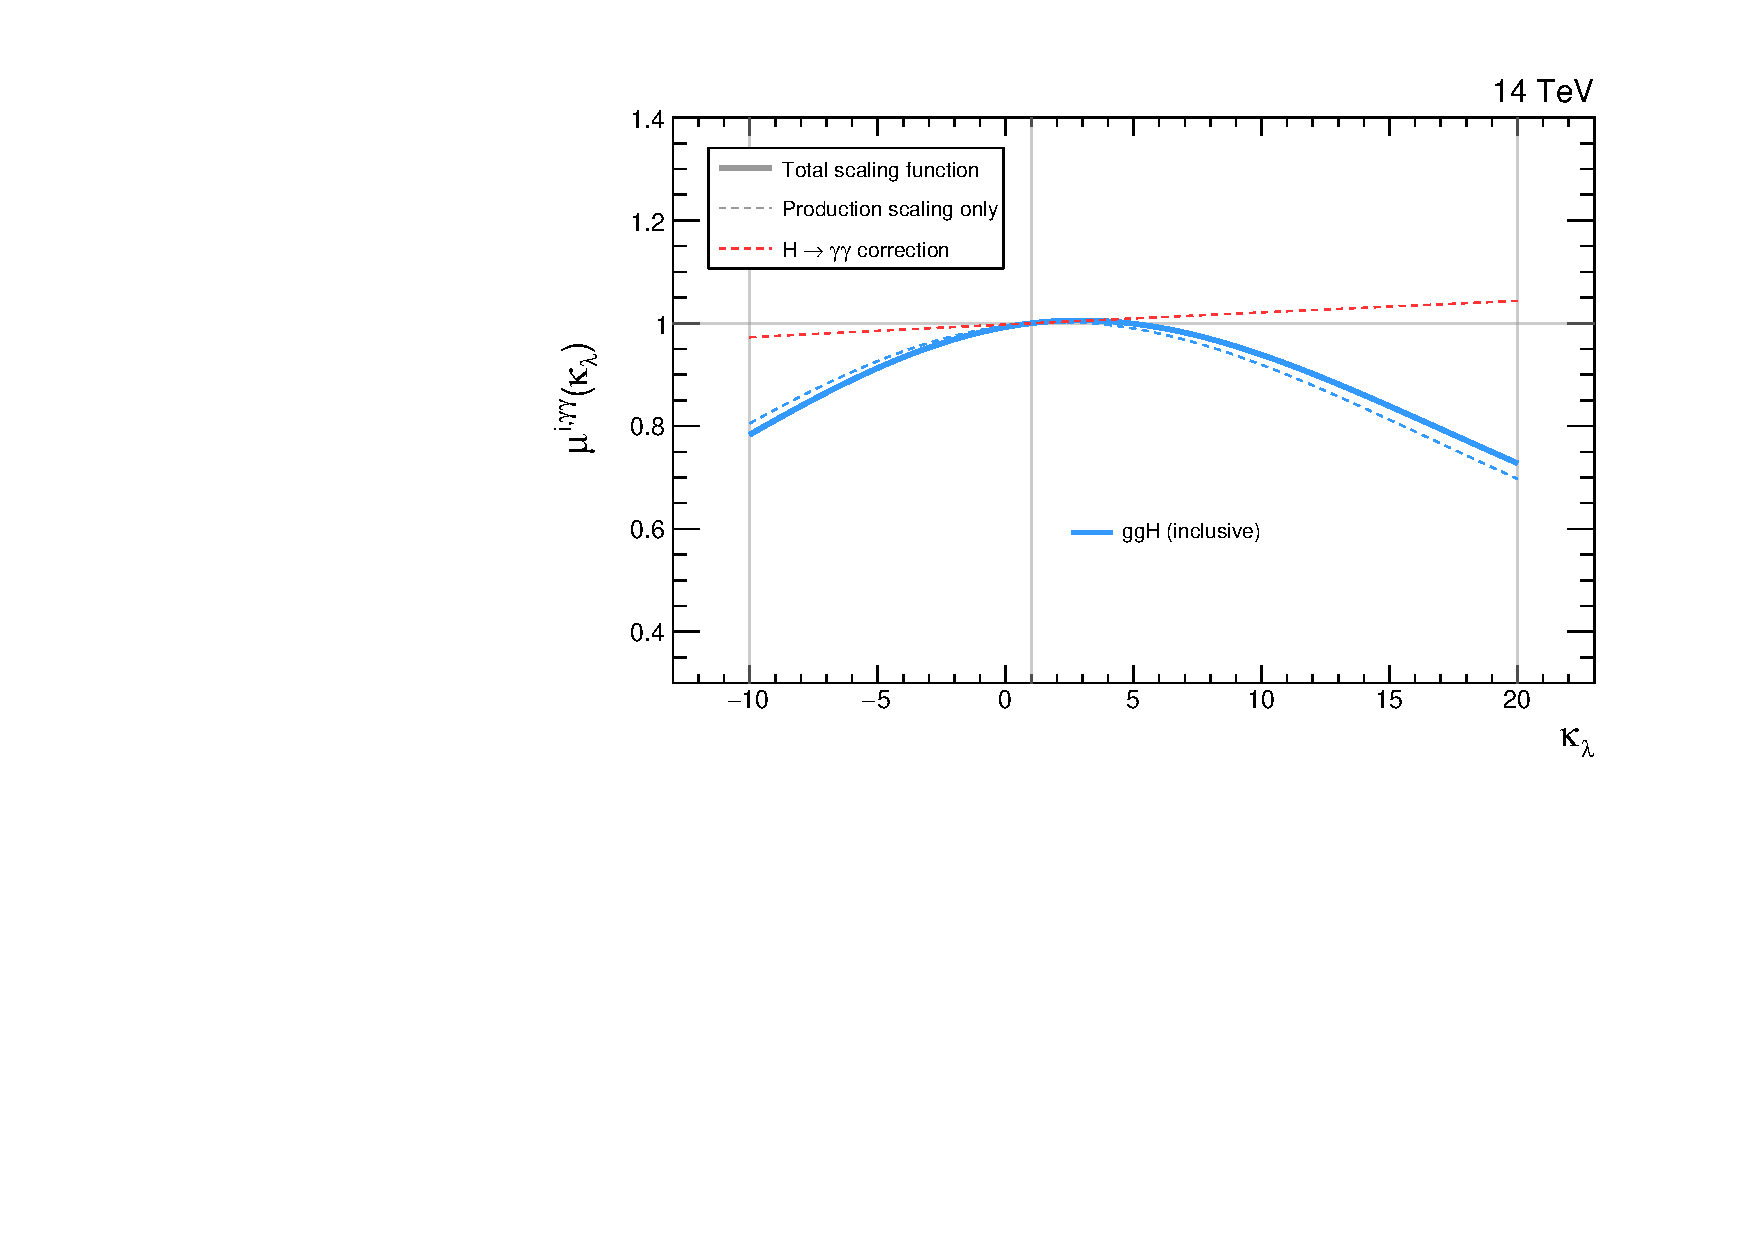
\includegraphics[width=.49\textwidth]{Figures/cms/trilinear/ggH.pdf}
  \caption[Scaling functions in terms of $\kappa_\lambda$]
  {
    Scaling functions, $\mu^{i,\gamma\gamma}(\kappa_\lambda)$, for the differential cross section times branching ratios targeted in this analysis. These are split into the different Higgs boson production modes. The ggH production mode uses an inclusive scaling function. In all plots, a lighter colour is used to represent lower $p_T^H$ bins. The total scaling functions including the correction from the \Hgg decay rate (red dashed line) are shown by the solid lines, whereas the affect on the production cross sections alone are shown by the dashed lines. All functions are plotted for the region of validity: $\kappa_\lambda \in [-10,20]$.
  }
  \label{fig:trilinear_sf}
\end{figure}

The $\kappa_\lambda$ dependence is largest (largest $C_1$ values) for ttH production at threshold (low $p_T^H$). For example, a 20\% enhancement to the ttH production rate for $p_T^H\in[0,45]$~GeV is predicted for $\kappa_\lambda \sim 10$. The horizontal dashed lines in Figure~\ref{fig:trilinear_dxs} correspond to the predicted values of the differential cross sections for anomalous values of the Higgs boson self-coupling: $\kappa_\lambda=10$ and $\kappa_\lambda=-5$. It can be seen that the expected uncertainties in the differential cross section measurements will enable $\kappa_\lambda$ to be constrained roughly between these values.

In order to extract the sensitivity to $\kappa_\lambda$, we make the substitution $\mu^{i,\gamma\gamma}\rightarrow\mu^{i,\gamma\gamma}(\kappa_\lambda)$ in the construction of the likelihood function, where $\mu^{i,\gamma\gamma}(\kappa_\lambda)$ are directly the scaling functions shown in Figure~\ref{fig:trilinear_sf}. As this represents an interpretation of cross section measurements, the theoretical uncertainties in the ttH~+~tH predictions ($\vec{\theta}^{\rm{th}}_s$) are directly folded into the measurement.

A scan of the profiled likelihood as a function of $\kappa_\lambda$~$(\equiv\alpha)$ is shown in figure~\ref{fig:trilinear_likelihood}. The scan is performed in the region $\kappa_\lambda \in [-10,20]$, beyond which the parametrisation becomes invalid as next-to-next-to-leading order (NNLO) effects become important. Additional likelihood scans are performed when only including the hadronic and leptonic categories, shown in red and purple, respectively. Clearly, both channels contribute significantly towards the final sensitivity. The constraints are tighter for negative values of $\kappa_\lambda$ since larger deviations in the ttH~+~tH differential cross sections are predicted, compared to positive values. The feature in the region around $5<\kappa_\lambda<15$ is a result of the turning points in the ttH scaling functions, which introduce a degeneracy into the parametrisation. This degeneracy is somewhat alleviated by the contamination of ggH in the signal model, which has a different scaling behaviour. Ultimately, the scan shows that with 3~\abinv of HL-LHC data, we can expect to exclude $\kappa_\lambda$ values outside of the range $-4.1<\kappa_\lambda<14.1$ at the 95\% confidence level using ttH~+~tH differential measurements in the \Hgg decay channel.

\begin{figure}[htb!]
  \centering
  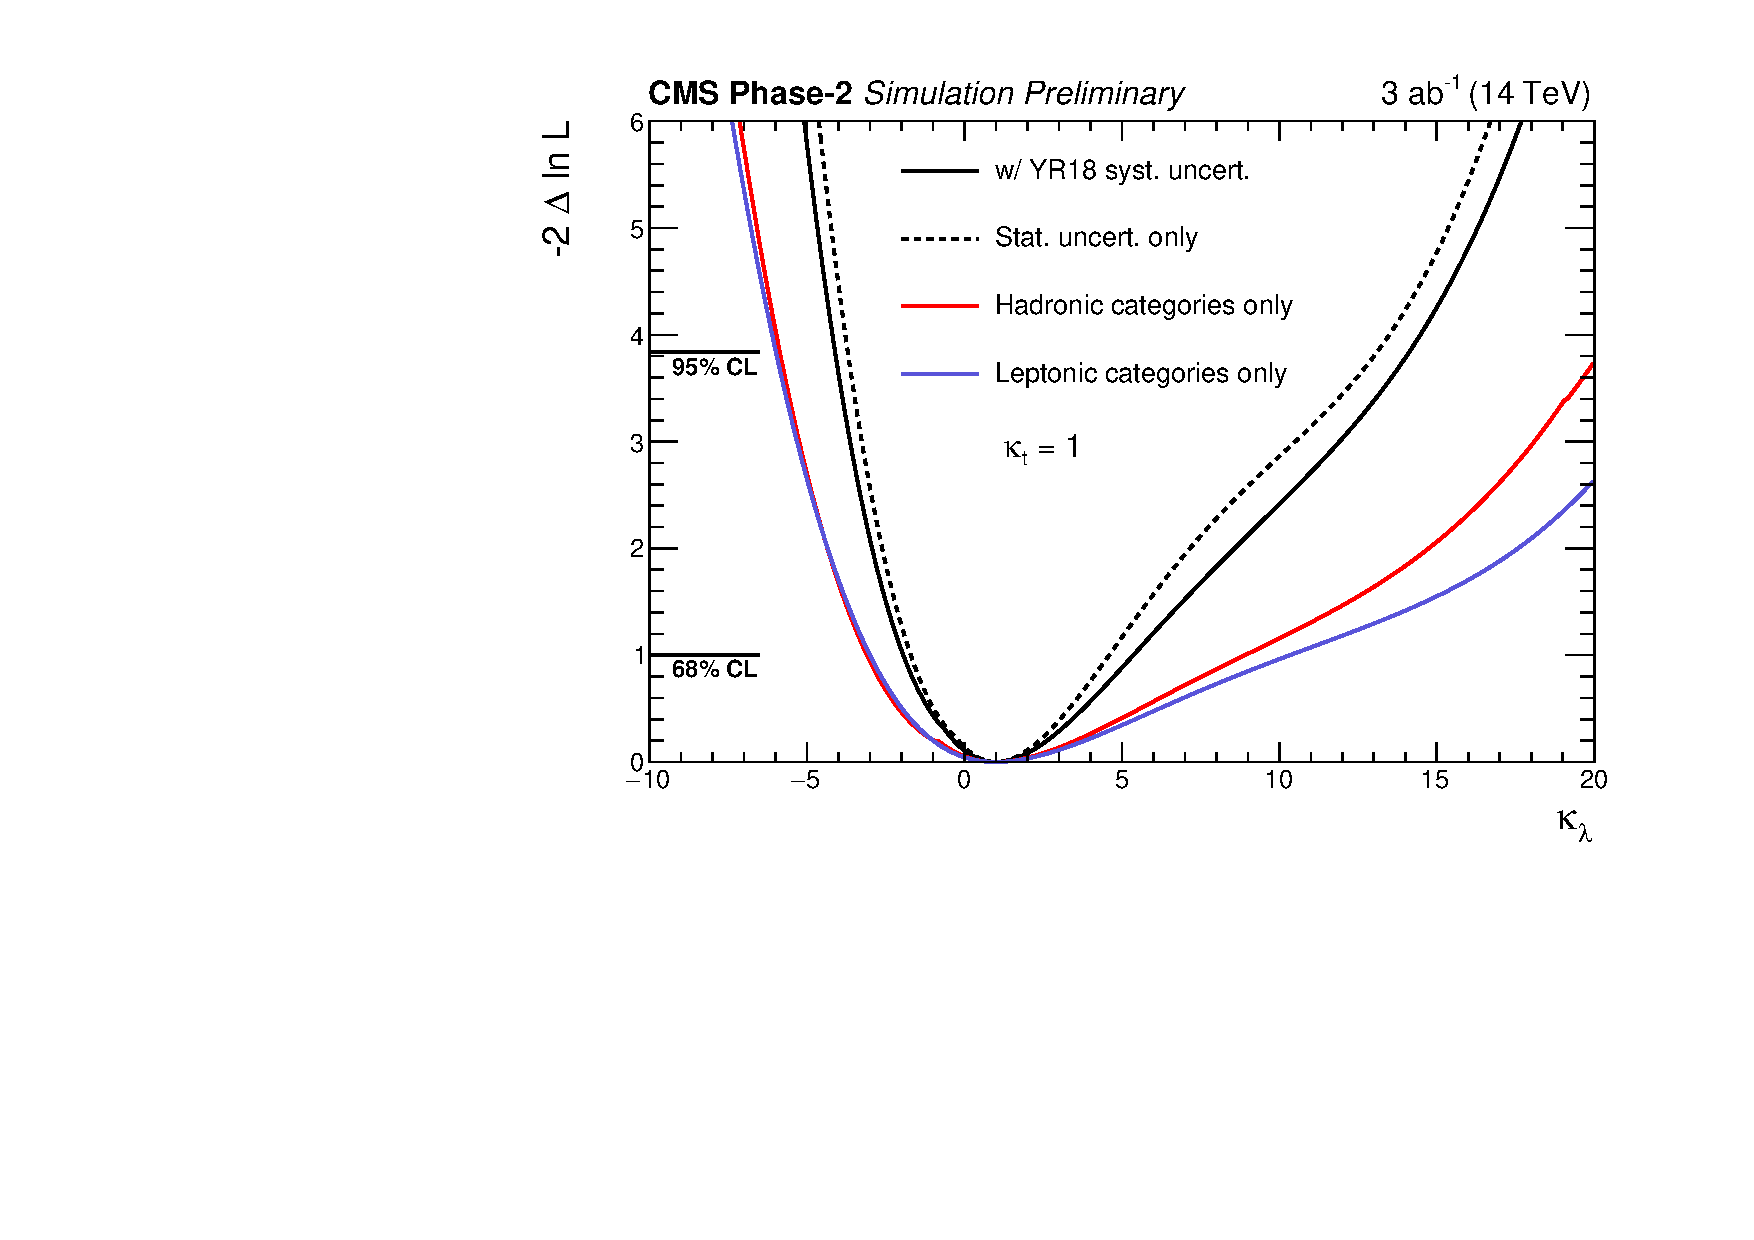
\includegraphics[width=.7\textwidth]{Figures/cms/trilinear/CMS-PAS-FTR-18-020_Figure_007.pdf}
  \caption[Likelihood curve for the $\kappa_\lambda$ fit]
  {
    The $q(\kappa_\lambda)=-2\Delta \ln L$ likelihood curve for the $\kappa_\lambda$ fit. The individual contributions of the statistical and systematic uncertainties are separated by performing a likelihood scan with all systematics removed. The observed deviation is dominated by the theoretical uncertainties in the Higgs boson cross section predictions. Additionally, the contributions from the hadronic and leptonic global categories have been separated, shown in red and purple, respectively.
  }
  \label{fig:trilinear_likelihood}
\end{figure}

An additional fit is performed in which an overall normalisation parameter for Higgs boson signal processes, $\mu_H$, is profiled. This parameter incorporates other BSM effects, such as an anomalous top-Higgs coupling, which in general cause an inclusive shift across the whole $p_T^H$ spectrum. Figure~\ref{fig:trilinear_2d} shows the results of a two-dimensional likelihood fit in the ($\kappa_\lambda,\mu_H$)-plane, in terms of the 68\% and 95\% confidence level contours. It can be seen that differential cross section measurements still provide sensitivity to $\kappa_\lambda$, without exploiting the overall normalisation of the $p_T^H$ spectrum. In other words, the shape of the spectrum is used to constrain $\kappa_\lambda$.

\begin{figure}[htb!]
  \centering
%   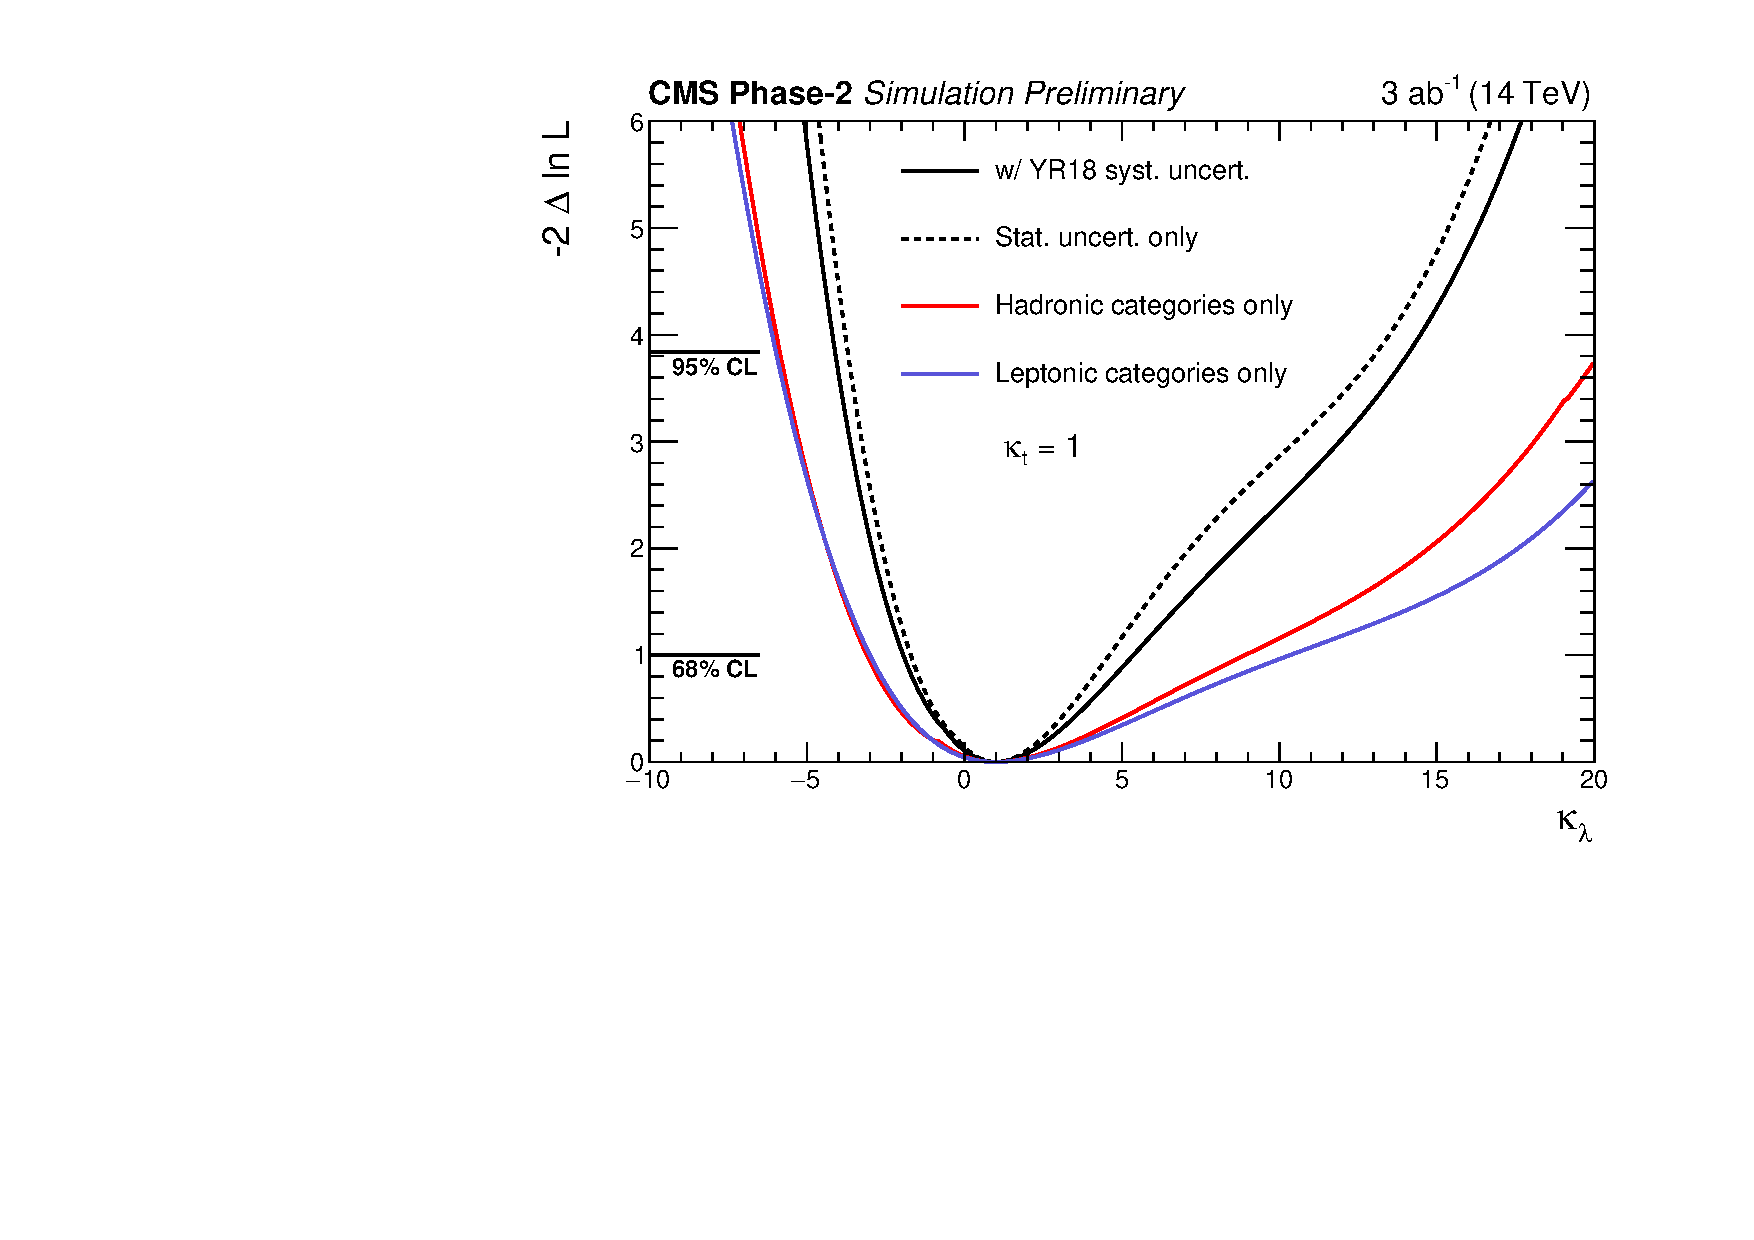
\includegraphics[width=.49\textwidth]{Figures/cms/trilinear/CMS-PAS-FTR-18-020_Figure_007.pdf}
  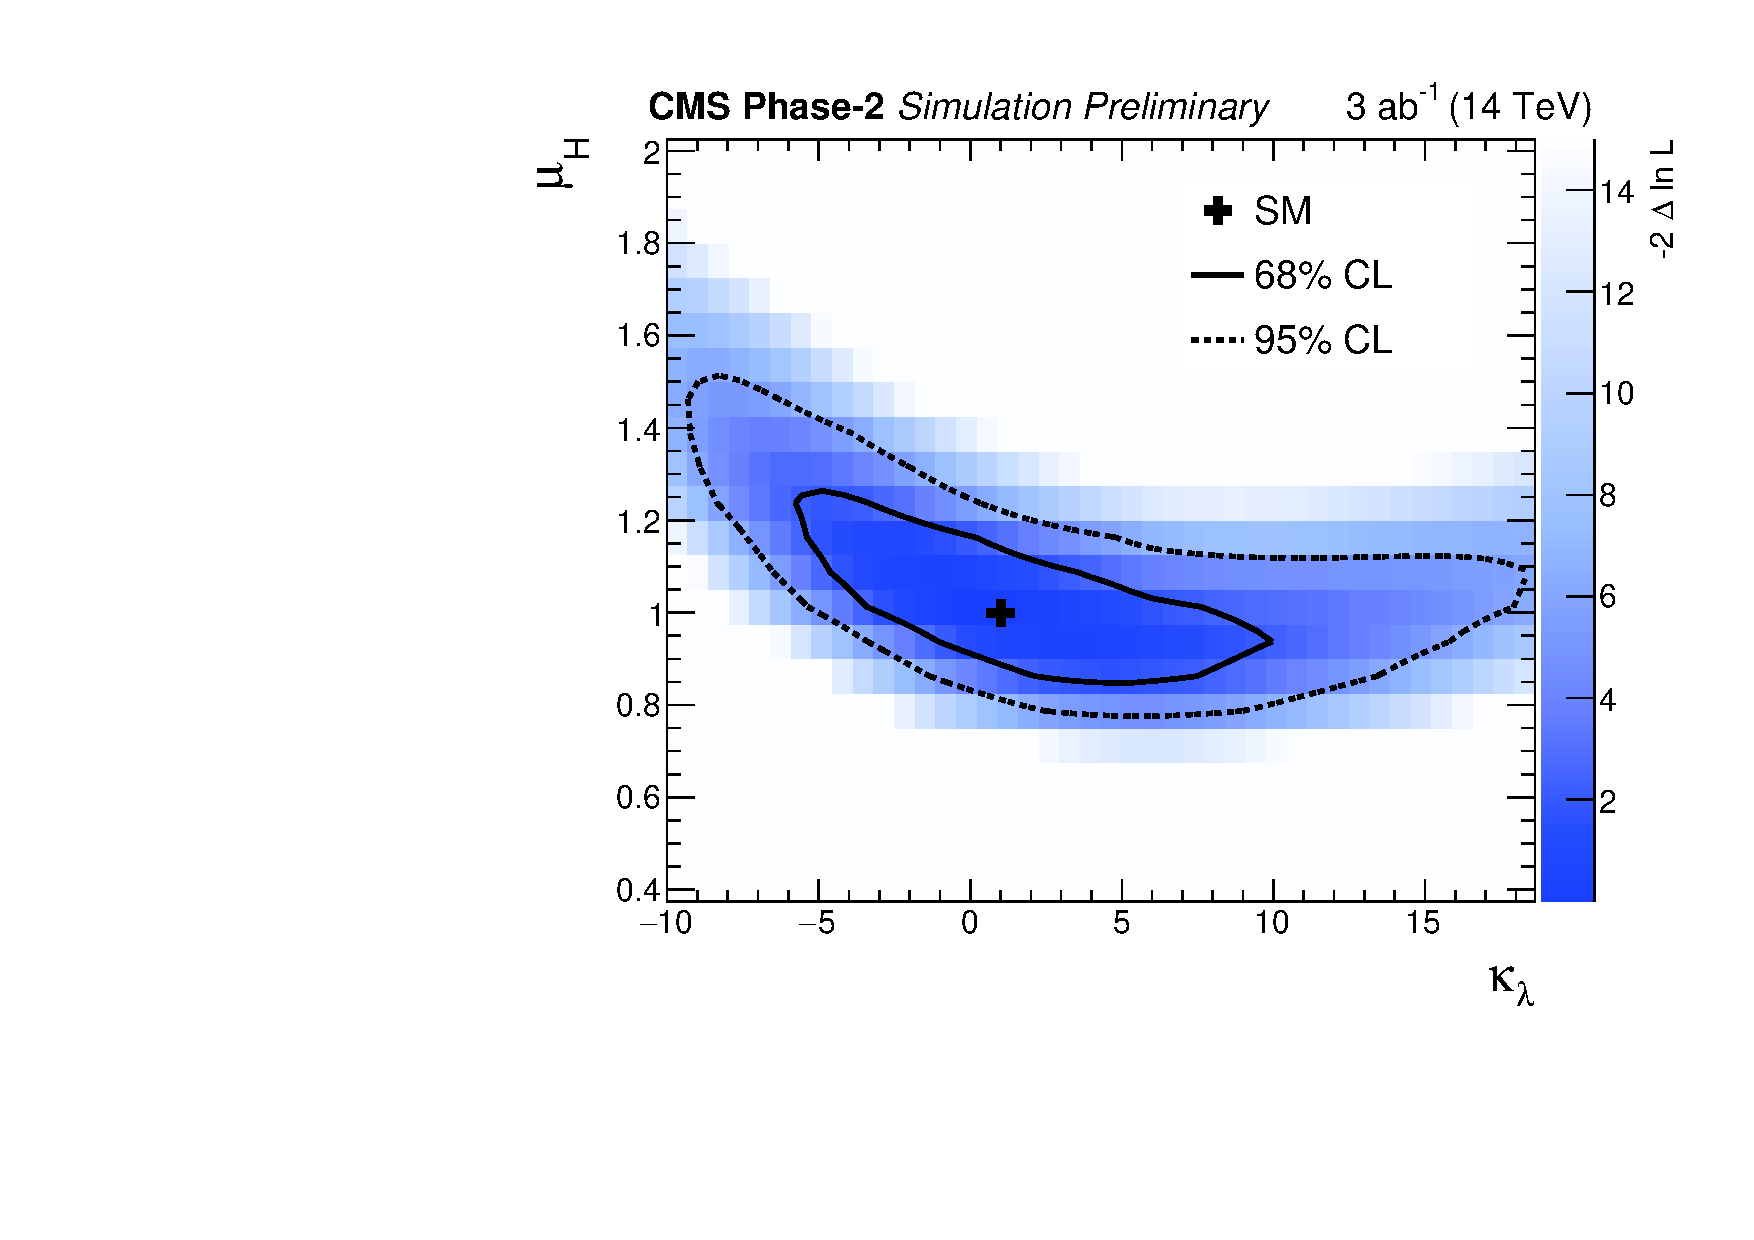
\includegraphics[width=.6\textwidth]{Figures/cms/trilinear/CMS-PAS-FTR-18-020_Figure_008.pdf}
  \caption[Two dimensional likelihood scan in $\kappa_\lambda$-vs-$\mu_H$]
  {
    The two-dimensional $q(\kappa_\lambda,\mu_H)=-2\Delta \ln L$ likelihood surface, where $\mu_H$ is an inclusive scaling parameter for all Higgs boson production modes. The SM expectation, 68\%  confidence level contour and 95\% confidence level contour are shown by the black cross, solid line and dashed line, respectively.
  }
  \label{fig:trilinear_2d}
\end{figure}

All in all, this analysis indicates that additional sensitivity to the Higgs boson self coupling is available through differential cross section measurements of single-Higgs boson production in association with top quarks. The expected sensitivity represents what could be achieved with 3~\abinv of HL-LHC data, in a \textit{single} Higgs boson decay channel (\Hgg). Of course, the ultimate sensitivity to the Higgs boson self-coupling at the HL-LHC will be achieved from a combination of similar analyses targeting the other Higgs boson decay channels and production modes, and with direct searches for di-Higgs (HH) production. The potential of these so-called \textit{global fits} are studied in detail in Ref.~\cite{DiVita:2017eyz}, where the addition of single-Higgs measurements are particularly important when considering deviations in other Higgs boson couplings.

\section{Summary}
The HL-LHC is a future operation of the LHC machine that will operate with instantaneous luminosities exceeding five times the nominal design value. The data taking phase of the HL-LHC is scheduled to begin in 2027 and will run for at least a decade, during which the LHC experiments will collect a huge amount of p-p collision data. This chapter has provided an insight into the HL-LHC project, particularly focusing on the areas of research that the author has been involved in. Firstly, the HL-LHC project was motivated and the experimental challenges from the increased levels of pileup were described. The CMS experiment will undergo a series of upgrades to maintain an excellent performance during the HL-LHC era. The upgrades to the CMS endcap calorimeters and the L1T were discussed. Section~\ref{sec:egid} introduced an ML algorithm to identify electron and photon showers from pileup-induced showers in the HGCAL L1T. The remainder of the chapter was dedicated to the physics reach of the HL-LHC, in terms of Higgs boson measurements. The expected sensitivity to differential cross section measurements of Higgs boson production in association with top quarks was outlined. These measurements were then shown to be sensitive to the Higgs boson self-coupling via radiative NLO corrections in single Higgs boson production. Measurements of this type will be complimentary to searches for HH production when extracting the ultimate constraints on $\lambda_3$ at the HL-LHC.